\section{单细胞 RNA-seq 数据下的细胞类型识别方法}
\label{sec:rafclust}

\subsection{引言}

基因调控与细胞类型密切相关 \cite{Hocker2020.09.11.291724,kang2020learning},
细胞聚类也是单细胞 RNA-seq 数据分析的热门和重要的问题, 
因此构建基因调控网络的一个不可或缺的前置任务是在单细胞数据集上对细胞的异质性进行聚类分析。
由于单细胞 RNA-seq 对于每个细胞测得的读数有限,细胞在测序过程中也会发生粘连,
因此导致每个细胞很多的基因表达量为 0,
这种现象被称之为单细胞的 dropout \cite{vallejos2017normalizing}。
同时,单细胞 RNA-seq 测序中将基因作为特征,常见的人和老鼠两种物种都有 20000 多个基因,
这种高维特征也给单细胞 RNA-seq 数据上的聚类带来挑战 \cite{stegle2015computational}。

在单细胞数据上的细胞类型识别上,除了聚类之外,还有一个十分具有挑战性的问题,即是如何从超大规模的 scRNA-seq 数据中识别稀有细胞。
稀有细胞代表了生物体内的次要细胞类型,当测序细胞的数量在数百个规模时,一个孤立的离群点 (singleton) 也很值得关注。
然而,随着吞吐能力的提高,研究重点转换到次要细胞类型的发现,再也不仅仅是单纯的单个细胞。
稀有细胞类型包括循环肿瘤细胞、癌症干细胞、循环内皮细胞、内皮祖细胞、抗原特异性 T 细胞、不变性自然杀伤性 T 细胞等。
尽管丰度较低,但稀有细胞群在决定癌症的发病机制、介导免疫反应、癌症和其它疾病的血管生成等方面起着核心作用。
抗原特异性 T 细胞对免疫学记忆的形成至关重要 \cite{slansky2003antigen,altman1996phenotypic,manzo2015antigen}。
内皮祖细胞,来源于骨髓,已被证明是肿瘤血管生成的可靠生物标志物 \cite{kuo2012dynamics,cima2016tumor}。
干细胞可以替代受损细胞,并用于治疗帕金森氏症、糖尿病、心脏病等疾病 \cite{jang2005stem}。
循环肿瘤细胞提供了前所未有的视角,为临床管理提供了实时的线索和根据 \cite{krebs2010circulating}。
现有的寻找稀有细胞的算法大部分依赖单细胞聚类方法,
在处理超大规模 scRNA-seq 数据时候非常耗时或者耗费内存。

本章中,我们提出了一种高效准确的单细胞聚类方法 RafClust。
针对当前单细胞 RNA-seq 数据集上细胞聚类不够准确鲁棒的问题,
本文使用多种相关性度量方法来刻画细胞的特征, 
然后使用随机森林回归模型进一步学习细胞与细胞之间的相似性矩阵,
基于相似性矩阵后采用层次聚类来决定细胞的最终类别。
实验结果表明,在十个单细胞数据集上, RafClust 在 ARI 上表现优于其它六种方法。

针对超大规模的 scRNA-seq 数据, 本文在 RafClust 方法的基础上进一步提出了一种高效准确的单细胞稀有细胞识别方法 DoRC (Discovery of Rare Cells)。
DoRC 产生的稀有度分数可以帮助生物学家们着重于下游分析,只对超大规模内的部分表达细胞 scRNA-seq 数据进行分析。
借助于单细胞聚类方法 RafClust,DoRC 可以进一步划分出准确的稀有细胞类型。
在超大规模的 scRNA-seq 数据 ${\sim}68$k 人血细胞的单细胞表达谱上,
 DoRC 在划分人类血液树突状细胞亚型方面有突出的效果, 执行效率高。
另外, DoRC 可以识别仿真数据集里面的稀有细胞,并且对细胞类型特征也很敏感。

\subsection{相关工作}

基于单细胞 RNA-seq 的细胞异质性研究主要是根据每个细胞的基因表达量来计算细胞之间的相似性,
结合聚类方法来确定细胞的类别。国内外研究者针对单细胞 RNA-seq 数据上的异质性研究已取得不少成果。
一类方法是最传统的聚类方法,比如使用 t-SNE 对数据进行降维然后使用 K-means 对数据进行聚类。
显然这种方法对噪声十分敏感。
Gr{\"u}n 等人 \cite{grun2016novo} 提出的 RaceID2 
使用 K-medoids 方法聚类,依据类内散布饱和临界值为依据确定分类个数。
另一类方法的研究思路是通过对原始数据进行插值处理 (imputation),减轻 scRNA-seq 数据中的 dropout 的影响。
典型的方法比如 Lin 等人提出的 CIDR 方法 \cite{lin2017cidr}。
CIDR 对 dropout 与基因表达值的关系进行了建模, 通过隐式插值处理后获取细胞与细胞之间的非相似性矩阵,
然后使用层次聚类获得最终的结果。
还有一类最流行的方法的研究思路是通过提高细胞与细胞之间的相似性计算的准确度和鲁棒性。
Kiselev 等人 \cite{kiselev2017sc3} 提出了一种共识聚类方法 SC3。
SC3 基于计算细胞与细胞间的 Pearson、Spearman 和欧氏距离三种不同相似性和主成分分析、拉普拉斯转换分别获得多个聚类结果,
然后通过计算这些聚类结果中两个细胞被聚为一类的数目来构建共识矩阵,
最后利用层次聚类获得最终的结果。
Wang 等人 \cite{wang2018simlr} 提出了无监督的 SIMLR 聚类方法。
SIMLR 构建不同粒度的高斯核矩阵来学习细胞与细胞之间的距离 (相似性) 矩阵,
并使用已有的比如 K-means 来获得每个细胞的类型。
Yang 等人 \cite{yang2018safe} 提出了聚合聚类方法 SAFE。
SAFE 选用了 SC3、CIDR、Seurat 和 t-SNE + K-means 四种聚类方法,
基于超图划分算法聚合四种聚类方法的结果。
Pouyan 等人 \cite{pouyan2018random} 提出了一种基于随机森林的计算细胞相似性的方法 RAFSIL。
RAFSIL 首先对基因过滤和聚类,接着对每个基因模块使用主成分降维,合并后作为随机森林的输入,
根据两个细胞落入同一颗决策树叶子上的数目计算细胞的相似性,然后使用层次聚类或者 K-means 获取每个细胞的类型。
相比于 SIMLR, RAFSIL 在聚类效果上有一定的提高,
但由于对基因聚类以及使用多颗决策树回归时,细胞数目一旦增加,计算效率显著降低。

scRNA-seq 技术的另外一个非常迫切和具有挑战性的应用,是从组织中的一堆细胞中捕获稀有细胞。
最近基于液滴 (Drop) 的单细胞转录组测序技术的发展,使得数以万计的单细胞的并行测序成为可能。
单个细胞的测序成本显著降低的情况下,稀有细胞的鉴别也变为可行。
迄今为止,已经有许多研究发表了可公开使用的转录组,细胞数量范围在 ${\sim} 20$k 和 ${\sim} 70$k 之间。
大规模的转录组样本通过削弱由于扩增阶段的失败所带来的影响,可以更好地捕捉到组织中的微小细胞亚群。
事实上,稀有细胞检测已经成为目前下游分析流程中的不可缺少的一环。
到目前为止,聚焦于研究怎样去检测稀有细胞转录组的算法还很少,
其中代表性的方法有 RaceID \cite{grun2015single}, GiniClust \cite{jiang2016giniclust} 和 FiRE \cite{jindal2018discovery}。
RaceID 涉及到计算成本十分高昂的参数模型,并用于检测离群的表达谱值。
它使用了 \textit{k}-means 聚类这种典型的基于距离的方法和间隙统计计算,
来作为识别大量细胞类型的中间步骤。
 GiniClust 使用了双管齐下的方法,
它首先使用 Gini 系数选择信息量大的基因,
然后它使用基于密度的空间聚类应用与噪声 (DBSCAN) \cite{ester1996density} 来发现离群细胞。
值得注意的是, RaceID 和 GiniClust 都使用聚类步骤来区分主要和次要细胞类型。
对于超大的 scRNA-seq 数据来说,速度非常慢,而且内存使用效率低。
相比之下, FiRE 为研究中的每一个细胞表达谱计算出一个稀有度分数。
它使用 Sketching 技术 \cite{wang2007sizing}来估计每个细胞的密度,
对于大规模细胞的低维编码来说, FiRE 运行速度非常快。

\subsection{基于随机森林相似性学习的单细胞聚类方法 RafClust}
\label{sec:method}

RafClust 方法对 scRNA-seq 数据进行细胞聚类,包括几个子步骤,如图 \ref{fig:rafclust} 所示, 这些步骤的细节将在下文中详述。
\begin{figure}[!htbp]
    \centering
    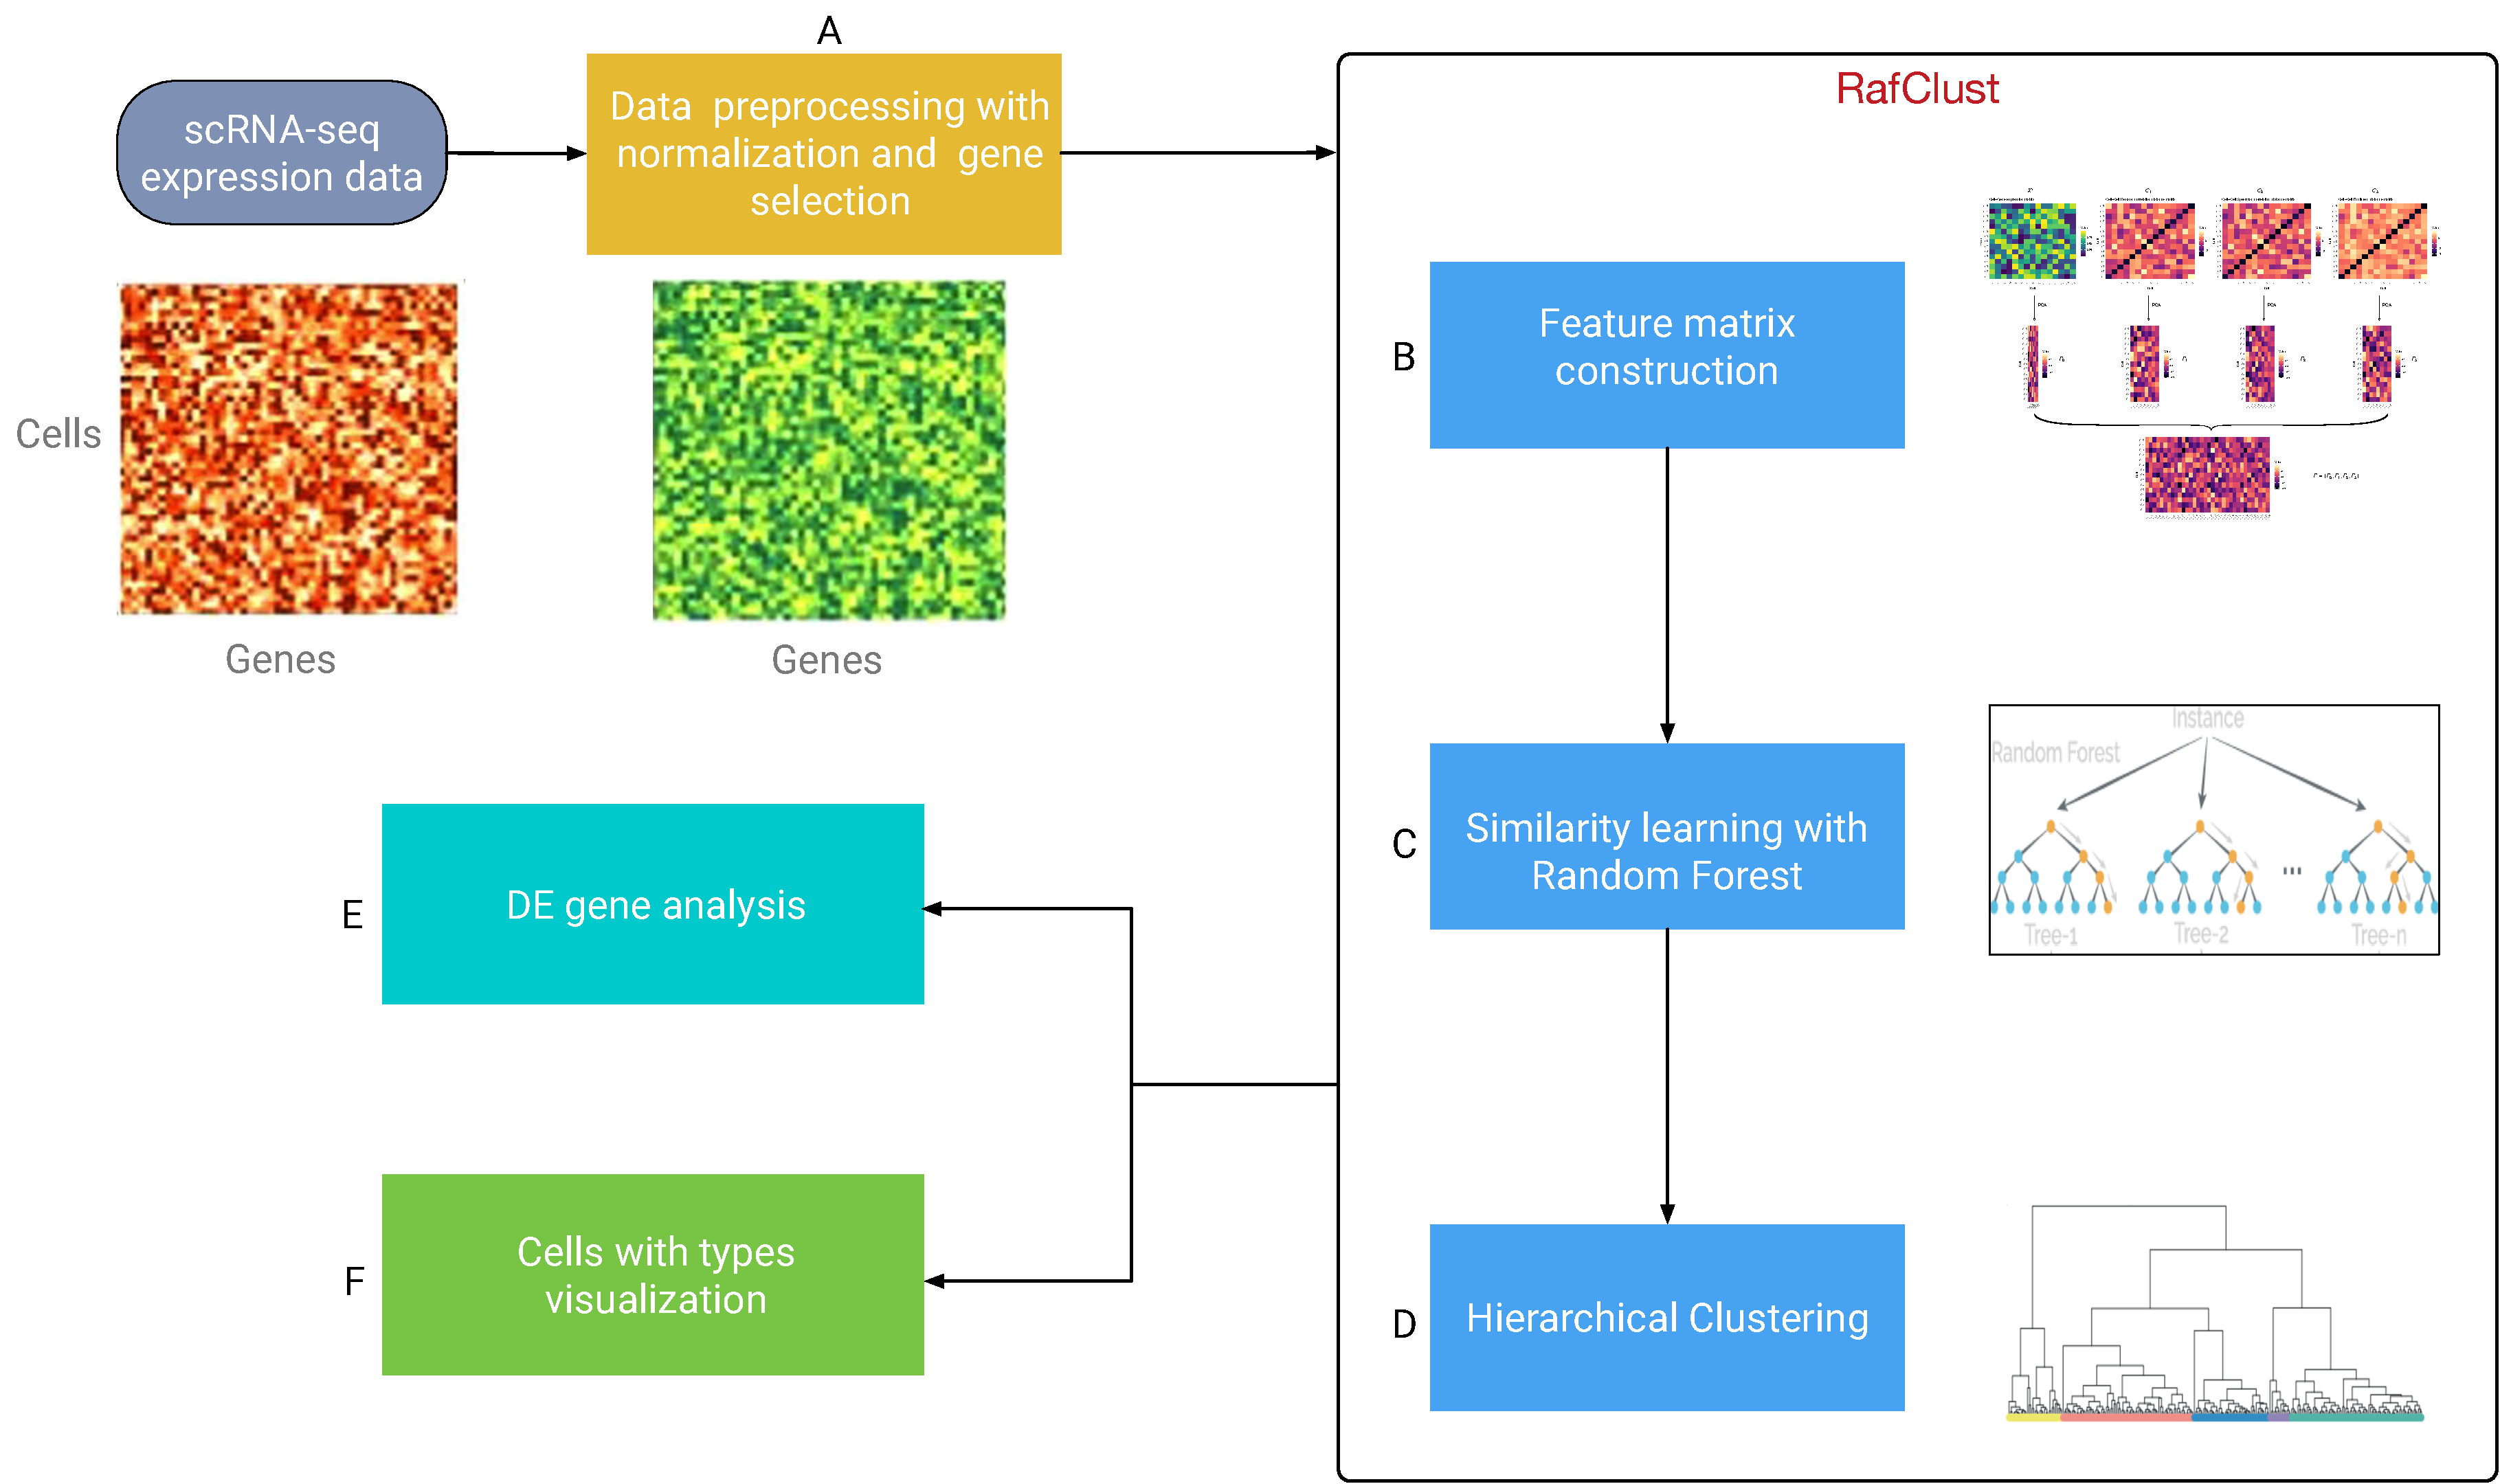
\includegraphics[width=0.95\textwidth]{flowchart-rafclust.pdf}
    \caption{RafClust 流程图。
    本图中的每个注释图代表了相应过程的输入或输出可视化。输入的是 scRNA-seq 表达数据二维矩阵,其中行代表细胞,列代表基因。
    (A) 用输入的表达数据进行数据预处理,输出的是一个归一化和列的维度缩减的矩阵。
    (B-D) RafClust 的核心程序。
    (B) 利用表达数据构造特征矩阵。
    (C) 利用随机森林算法来学习细胞与细胞的相似性矩阵。
    (D) 利用层次聚类来对细胞进行聚类。
    (E) 对不同类型的细胞进行不同的差异基因分析,从而得到细胞类型的特异基因。
    (F) 细胞表达数据与其类型可视化,在基于 t-SNE 的二维图中不同的颜色代表不同的细胞类型。
    }
    \label{fig:rafclust}
\end{figure}

\subsubsection{数据规范化和基因选择}
\label{subsec:datapreprocessing} 

本文假设归一化的 $n$ 个细胞的基因表达数据 (观测值), 每个细胞含有 $p$ 个基因(特征),
组成一个 $n \times p$ 的表达式矩阵 $X=\left(x_{1}, x_{2}, \ldots, x_{n} \right)^ T$。
其中 $x_{i}$ 表示 $p$ 基因在细胞 $i$ 中的表达值。
$x_{i}=\left(x_{i1}, x_{i2},\ldots, x_{ip} \right)$。
矩阵 $X$ 在加上 1 的伪数 (pseudo-count) 后进行对数变换,即 $X^{\prime} = log_2 (X + 1)$。
然后,如果基因在细胞总数中的表达低于一个预定频率 $\beta$,则该基因会被过滤掉。
默认情况下, $\beta$ 设置为 0.06 \cite{kiselev2017sc3}。 
基因过滤的动机是,除了保守的基因外,其它一些很普通的甚至是低表达的基因往往对细胞的聚类没有贡献。

\subsubsection{细胞类型识别}
\label{subsec:rafclust} 
为了从稀有细胞集合中确认不同的细胞类型,本文提出了一种无监督的基于随机森林的相似性学习算法,命名为 RafClust。
类似于其它的许多方法 \cite{kiselev2017sc3,pouyan2018random,mohammadi2018geometric,sinha2018dropclust,Srinivasan511626,Li530378,zheng2019sinnlrr},
RafClust 也是两个步骤的方法,
第一个步骤是使用随机森林进行相似度学习 (相似性学习步骤, similarity learning),
第二个步骤中使用层次聚类 (聚类步骤, clustering)。
在相似度学习步骤中,一个非常关键的预处理程序是特征矩阵的构建。
稀有细胞 (rare cells) 与丰富细胞 (abundant cells) 不同,本文将使用细胞和细胞的尽量多的不同类型的相似性,来充分刻画稀有细胞的本性特征。
因此,在基于基因过滤后的表达矩阵 $X^{\prime}$ 上,
本文利用欧几里德 (Euclidean)、皮尔逊 (Pearson) 和斯皮尔曼 (Spearman) 指标分别计算出三种不同的细胞-细胞距离矩阵 $\{C_1, C_2, C_3\}$。
然后将主成分分析 PCA 应用于每个距离矩阵,也应用于 $X^{\prime}$ 上,来减少数据维度的同时也去除其本能噪声。
每个矩阵中信息量最大的成分由``elbow 法" \cite{thorndike1953belongs} 保留,
这样就共计产生了 $\left\{ {F}_{i} \in \mathbb {R} ^ {n \times m_{i}} \right\}_{i = 0}^{3}$ 四个矩阵。
最终的特征矩阵 $F$ 由这些矩阵按行拼接组成, 行代表细胞, 列代表手工特征 (handcrafted features)\footnote{区分于现在比较流行的深度学习里的 auto-learned features}。
\begin{equation}
\label{lab:f}
{F} = ({F}_{0}, {F}_{1}, {F}_{2}, {F}_{3})
\end{equation}

$F$ 中的列数 (维度) (即特征总数 $\tilde {p} = \sum_{i = 1}^{k} m_{i}$) 与数据有关。
和细胞 $j$ 现在用特征向量 $f_{i} \in \mathbb {R} ^ {\tilde{p}}$ 表示。
显然,$F$ 既反应了细胞的自身表达值,也包含了细胞与其它细胞的相似性关系特征。
接着,我们利用特征矩阵 $F$ 来进行基于随机森林 (RF) 的相似性学习。
图 \ref{fig:rafsim} 是一个示例,在大小为 $15 \times 15$ 基因表达矩阵的数据集上来说明整个特征矩阵的构建步骤。

% \begin{figure}[!htbp]
%   \begin{adjustbox}{addcode={
%     \begin{minipage}{\width}}{
%         \caption{一个有 15 个细胞和每个细胞 15 个基因的示例数据集中手动制作的特征矩阵构造。
%         最终的特征矩阵 $F$ 在这个示例中是 $15\times34$ 维度大小的。}
%         \label{fig:rafsim}
%     \end{minipage}},rotate=90,center}
%     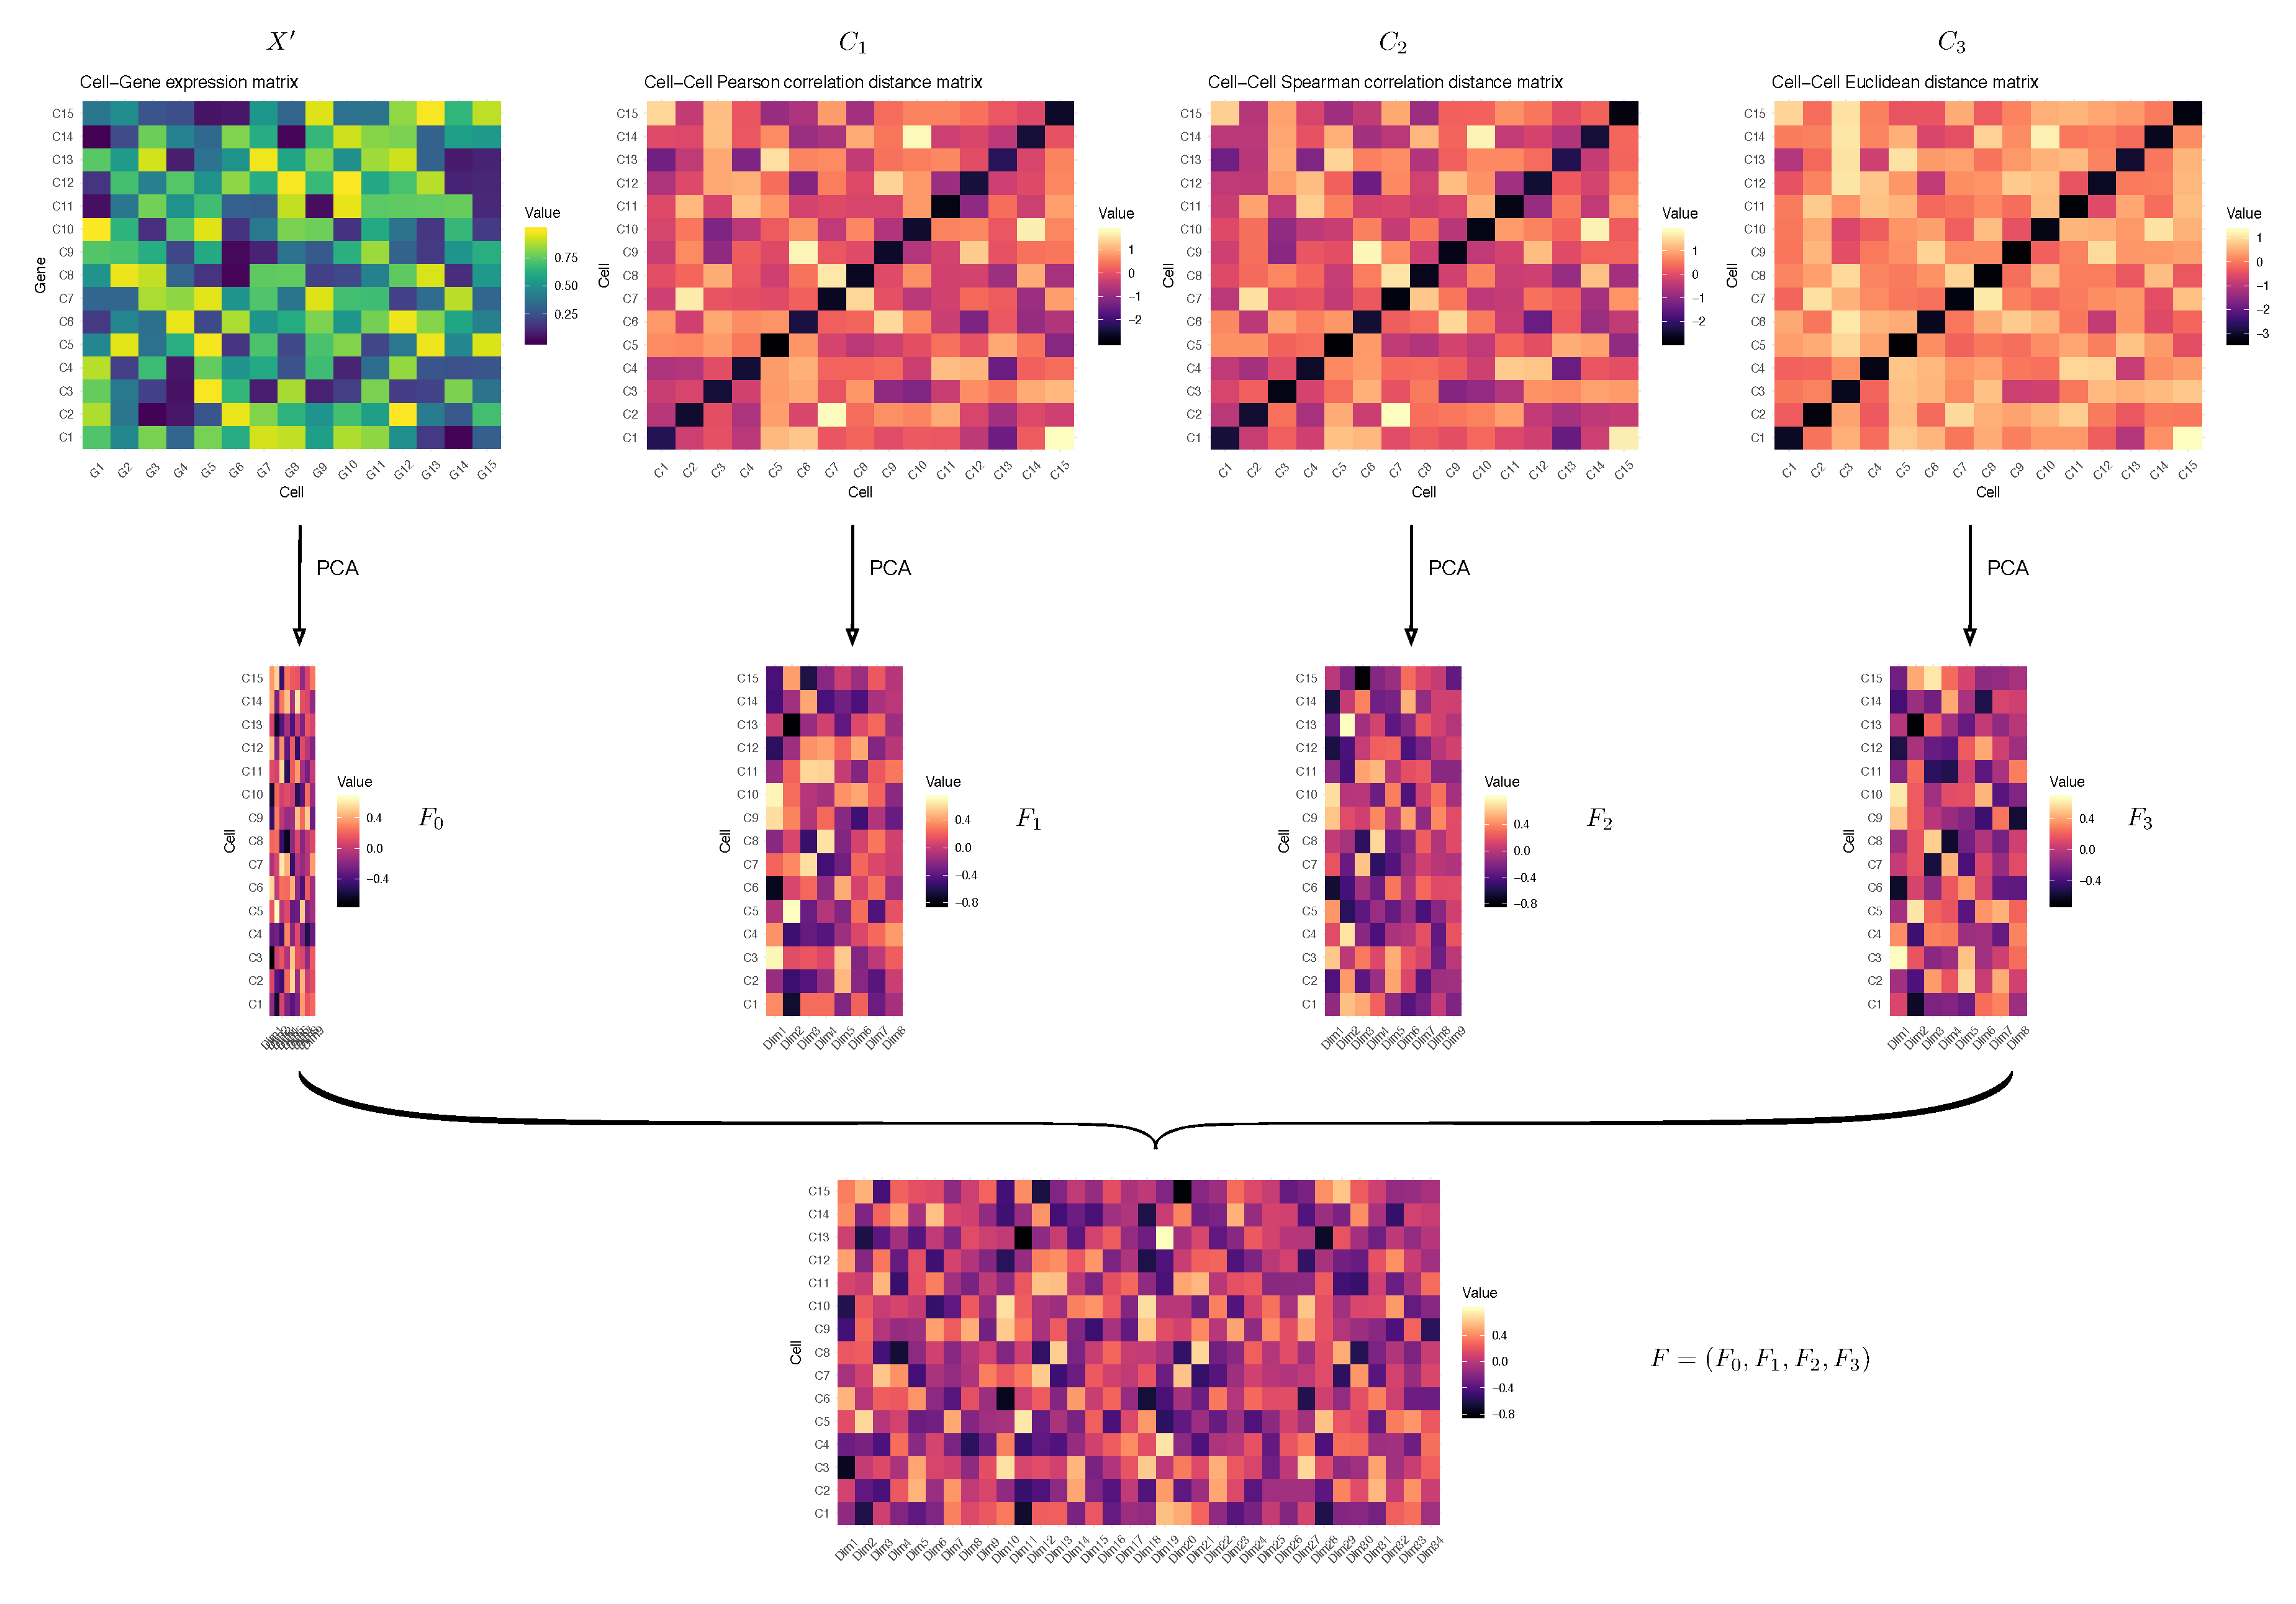
\includegraphics[scale=.42]{rafsim.pdf}%
%   \end{adjustbox}
% \end{figure}
\begin{figure}[!htbp]
    \centering
    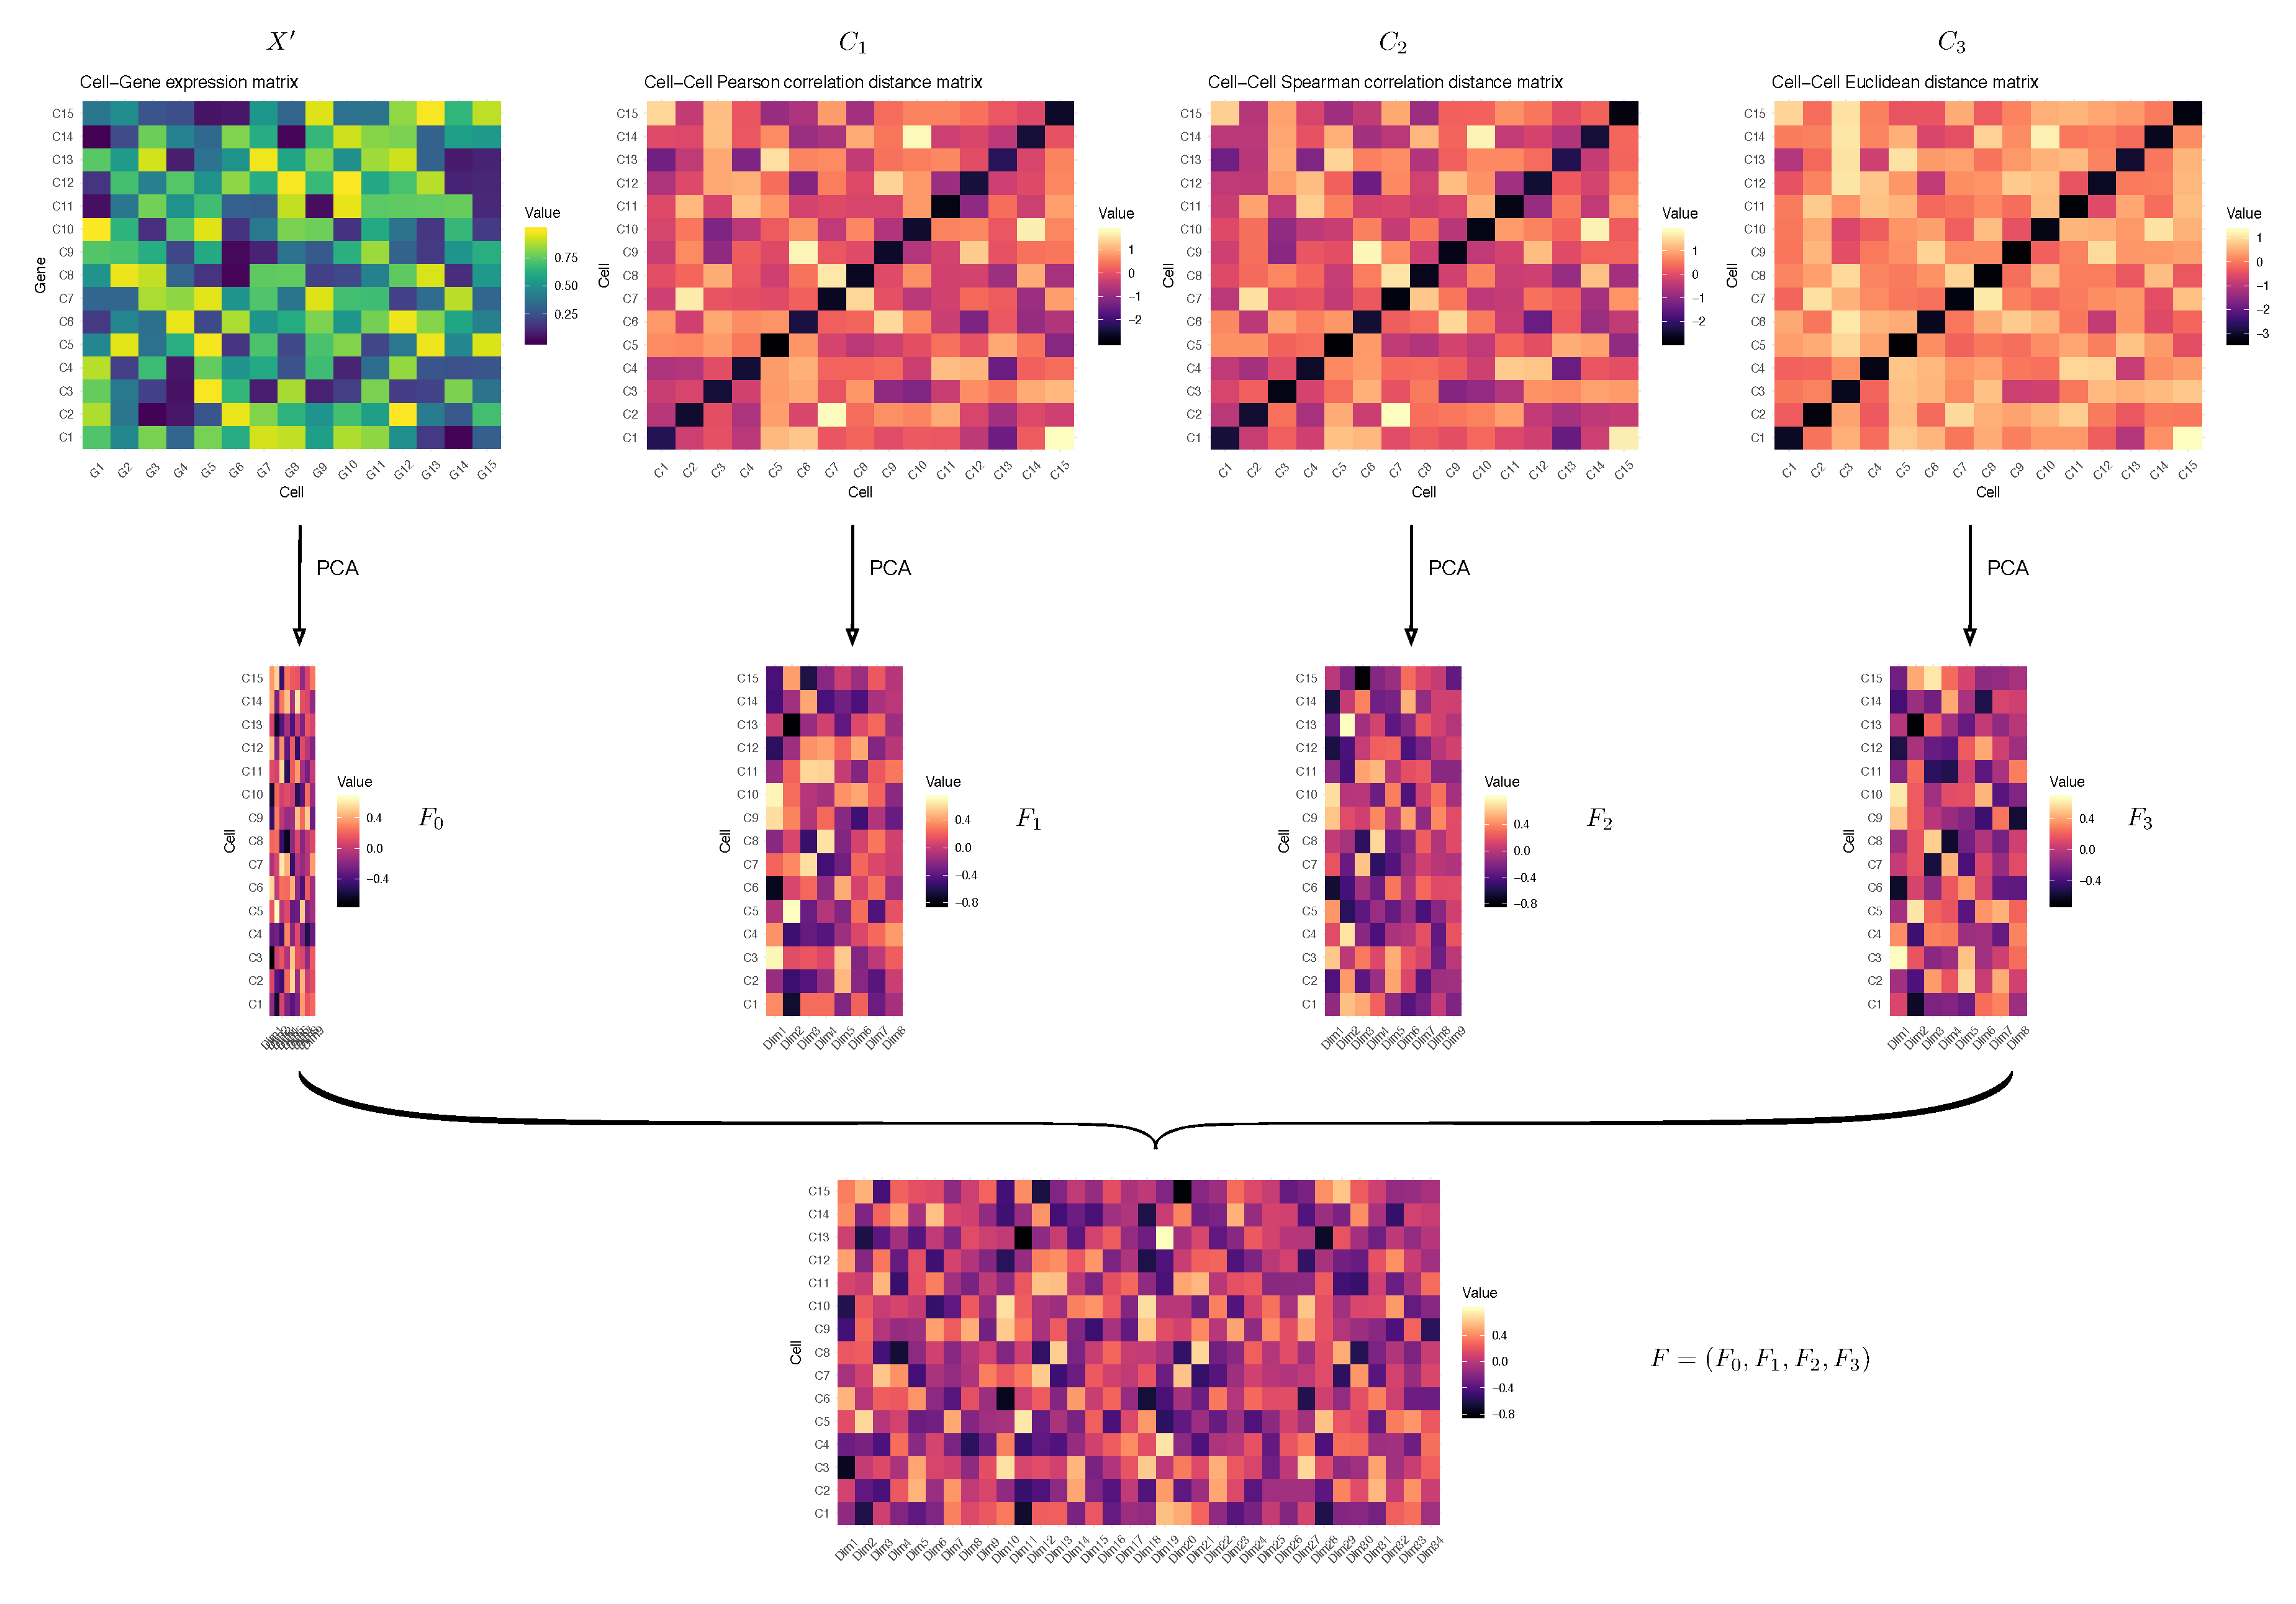
\includegraphics[width=0.9\textwidth]{rafsim.pdf}
    % \caption{Illustration of the hand-crafted feature matrix construction in a toy dataset with 15 cells and 15 genes. 
    % The final feature matrix $F$ is in a $15 \times 34$ shape in this case}
    \caption{
        一个有 15 个细胞和每个细胞 15 个基因的示例数据集中手动制作的特征矩阵构造。
        最终的特征矩阵 $F$ 在这个示例中是 $15\times34$ 维度大小的。
    }
    \label{fig:rafsim}
\end{figure}

RF (随机森林, Random Forest) 是一种应用非常广泛的基于决策树的分类和回归方法 \cite{breiman2001random}。
它也可以用无监督的方式来推断对象之间的相似性 \cite{shi2006unsupervised,breiman2011manual,pouyan2018random}。
基于 RF 的相似性学习方法很容易适应于并行计算,
对离群值具有鲁棒性,内在具有特征选择的特性,这三个特点特别适合用来分析高维和噪声数据,
特别是类似于单细胞 RNA 测序图谱数据。
本文按照以下步骤来学习细胞-细胞的相似性。
在选择一个单一的特征 $j$ (特征矩阵 $F$ 中的第 $j$ 列) 后, 
我们使用围绕质心点进行划分的算法 PAM (partitioning around medoids),估计类别的数量并得到对应于类别的伪标签。
与 K-means 聚类算法相比, PAM 对孤立点不敏感。
%我们直接使用 R 包 fpc \cite{package-fpc}中的 \textit{pamk} 函数来获取该特征 $j$ 的向量中的类标签。
然后,我们从 $F$ 中去掉第 $j$ 列,并且使用 RF 对缩减后的数据集 $F_{-j}$ 进行对伪标签的回归学习。
让 $f_p$ 表示 $F_{-j}$ 的第 $p$ 行,
如果 RF 包含 $N$ 颗树,并定义 $nt(f_p,f_q)$, 作为通过同一片叶子对细胞 $f_p$ 和 $f_q$ 进行归类的树的数量。
基于 RF 的 $n \times n$ 相似度矩阵 $S_j$ 是通过以下方式定义:
$S_{j_{pq}} = nt(f_p,f_q) / N, 1 \le p,q \le n$。
%我们使用 R 包 randomforest \cite{package-randomforest},其默认森林大小为 500 棵,即 $N=500$。
对所有的 $\tilde{p}$ 特征重复这个过程,得到 $\tilde{p}$ 相似度矩阵 $S_j$,$j=1,2,\ldots,\tilde{p}$。
通过对所有 $S_j$ 进行平均,得到最终的细胞-细胞相似度矩阵 $S$,
并通过 $D=1-S$ 得到距离矩阵 $D$。

接下来,对距离矩阵 $D$,使用层次聚类中的平均连锁聚类方法 (average linkage clustering) 来对细胞进行聚类,
使用了来自 R 包 dynamicTreeCut \cite{langfelder2007defining,package-dynamicTreeCut} 的 \textit{cutreeDynamic} 函数自动确定细胞的类别,
并为每个细胞分配正确的类标签。
另外,我们还提供了使用 R 包 dynamicTreeCut 中的 \textit{cutree} 函数来支持用户自定义细胞的类别数。

\subsubsection{差异基因分析}
\label{subsec:de}

使用 RafClust 得到了细胞的类别标签后,
本文采用 NODES \cite{Sengupta049734} 这一快速的非参数化、差异化表达 (DE) 分析工具进行差异基因分析。
NODES 被证明比传统的基于批量细胞测序的差异分析方法 DESeq2 \cite{love2014moderated}、edgeR \cite{robinson2010edger},
以及针对单细胞的差异表达分析方法 scde \cite{kharchenko2014bayesian} 和 Wilcoxon 秩和检验 (Wilcoxon rank sum test) 都有效 \cite{Sengupta049734}。
以 0.05 作为 FDR (False Discovery Rate) 的阈值, FC (fold change) 变化(也就是两个组间表达量的比值) 阈值默认为 log2(5)。
在 DE 基因中,在特定类中相对于其余各类显著上调的基因被命名为细胞类型特异基因。


\subsection{基于孤立森林的单细胞稀有细胞识别方法 DoRC}
\label{sec:method}

RaceID 和 GiniClust 都依靠无监督聚类来检测稀有细胞。
RaceID 中的 \textit{k}-means 聚类是基于距离的,
而 GiniClust 中的 DBSCAN 聚类是基于密度的。
它们都属于基于近邻的方法进行离群点检测。
基于近邻的方法假设一个离群样本与其最近邻的接近程度与该样本与数据集中大多数其它样本的接近程度有很大的差异。
聚类性能通常取决于一些参数敏感性且工作效率低下,因为不同分布的数据点之间的近似度不同。
另一个主要问题是,样本聚类的分辨率 (resolution) 问题。
一般来说,多级聚类变得至关重要,因为次要的类经常在首次筛选就被过滤掉了 \cite{campbell2017molecular}。
其它主要细胞类型会影响数据集中的表达差异,
特别是在处理大型 scRNA-seq 数据集时,情况变得更加糟糕。

为了解决上述问题,本文提出了一种从超大规模 scRNA-seq 数据中快速准确检测稀有细胞的方法,
命名为 DoRC。
DoRC 的灵感来自于我们观察到,稀有细胞在单细胞数据集里往往是``少而不同", 这跟机器学习里的样本孤立性十分契合。
孤立森林可以充分捕捉稀有细胞的特征,
其中,每个细胞的稀有性是以树枝的聚合长度为特征的。
一个细胞的聚合长度越长,该细胞与其它细胞区分的因素就越多,它成为稀有细胞的可能性就越大。
从数量上看,孤立森林中的聚合异常分数在本质上反应了稀有特性,
这为我们调查和进一步决定细胞的稀有性提供了基础。

DoRC 方法是用于从超大型 scRNA-seq 数据中发现稀有细胞,包括若干个子步骤,如图 \ref{fig:flowchart} 所示。
% \subsubsection{}
% \label{subsec:datapreprocessing} 
其中,预处理部分包括数据规范化和基因选择。
每个数据集上,在至少 3 个细胞中读数超过 2 的基因被保留用于下游分析,
然后使用中位数归一化。
除 \textit{Splatter\_500} 之外的其它数据集,
本文基于基于它们的相对分散度 (dispersion,即方差/均值) 与具有相似平均表达量的基因之间的预期分散度 \cite{zheng2017massively,macosko2015highly}选出 1000个变化最大的基因。
最后,将处理后的伪计数矩阵 (pseudo-count) 加 1 后进行对数变换。
对所有的数据集进行了预处理之后,后续的关键的处理步骤在下文中将详细讲述。

\begin{figure}[!htbp]
    \centering
    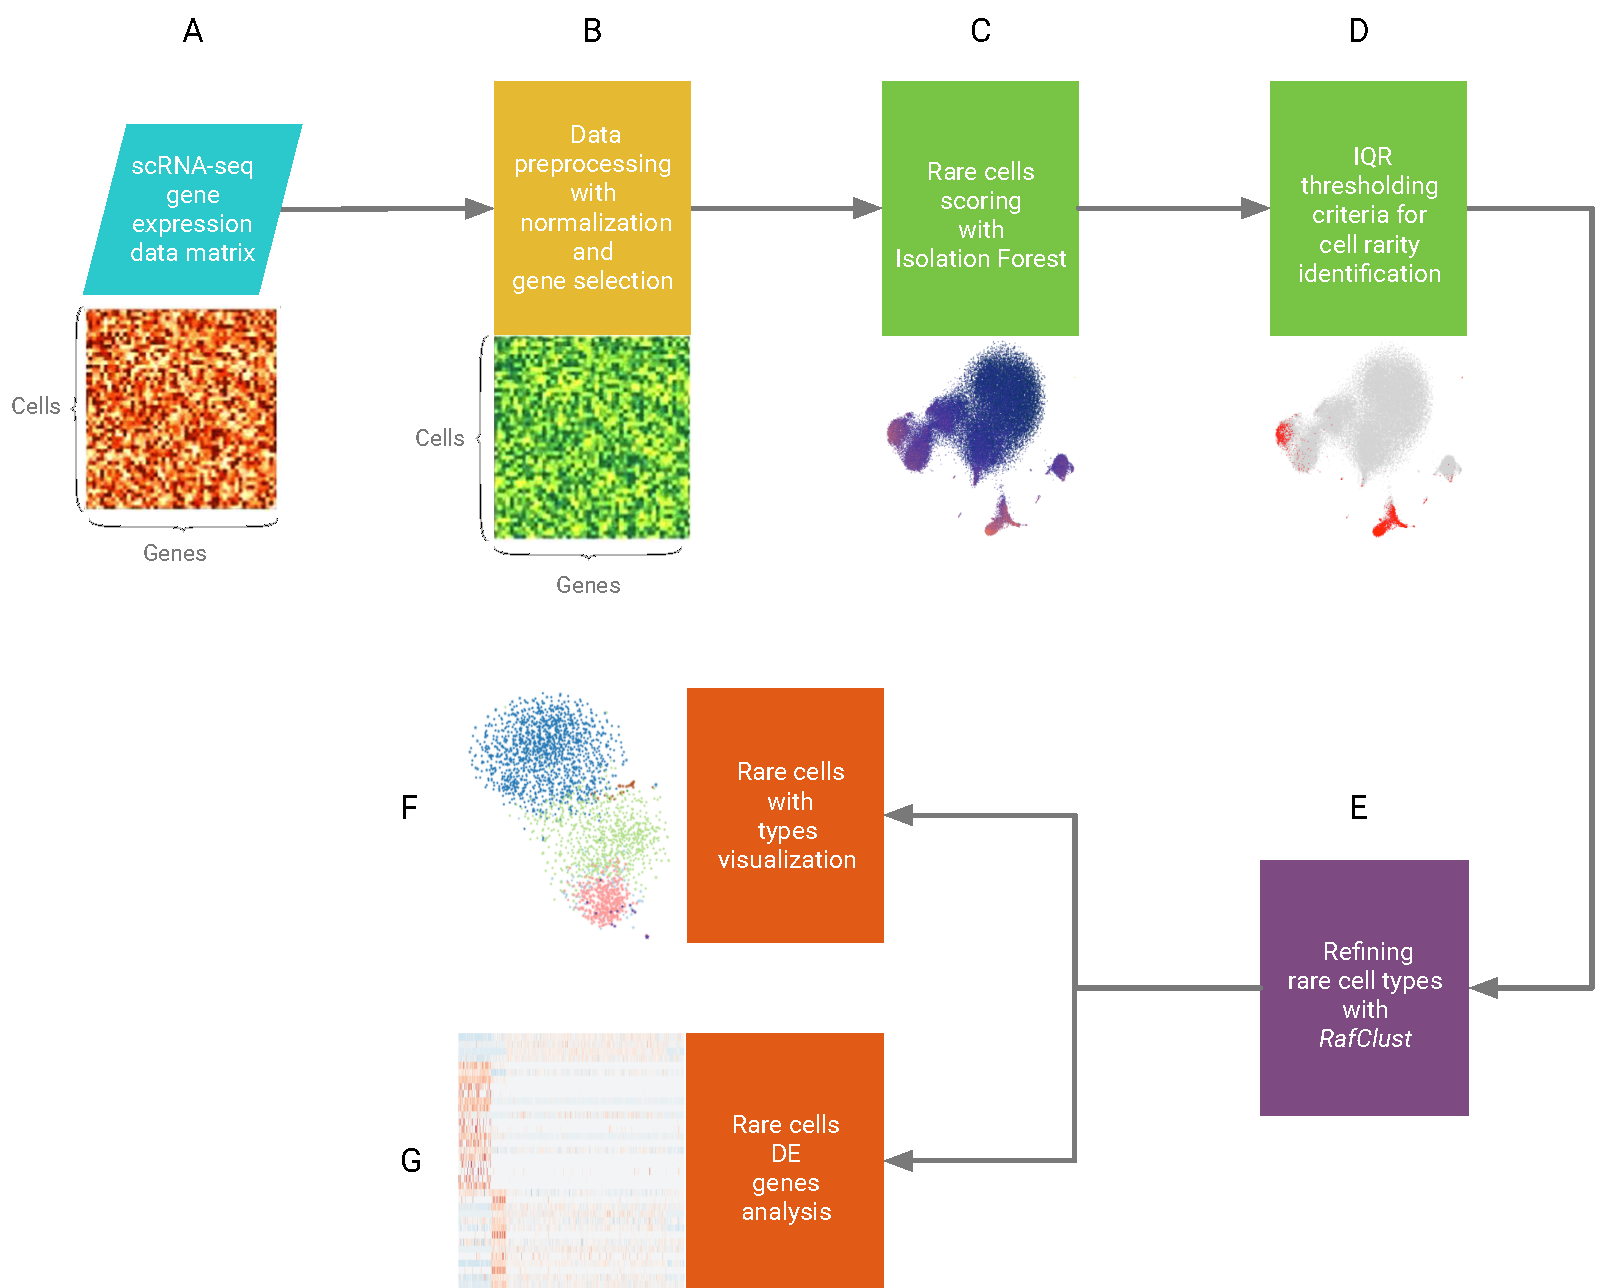
\includegraphics[width=\linewidth]{flowchartv4.pdf}
    % \caption{DoRC flowchart. The flowchart illustrates the processes of our proposed DoRC method for rare cells detection from ultra-large scRNA-seq data. 
    % Each annotated vignette in this figure represents the input or output visualization for the corresponding procedure. 
    % (A) The input is the scRNA-seq expression data 2D-matrix, whose row stands for cells, column for genes, respectively.
    % (B) Data preprocessing with the input expression data, the output is  a normalized and the column dimension reduced matrix. 
    % (C-D) Rare cells discovery with Isolation Forest, which are the workhorse procedures of DoRC. 
    % (C) Rare cells scoring with Isolation Forest, the output is a list of continuous anomaly scores for all the cells.
    % The scores can be visualized in the t-SNE-based 2D plot of the dataset; 
    % (D) IQR thresholding criteria for cell rarity identification, the binary annotations are also visualized in the t-SNE-based 2D plot.
    % (E) Refining rare cell types with RafClust. Notably, this sub-procedure is optional if we do not care about the types of rare cells.
    % (F) Rare cells with types visualization, different colors represent different rare cell types in the t-SNE-based 2D plot of the rare cells.
    % (G) Different expression genes analysis with different types of rare cells, the cell type specific genes are consequently obtained. 
    % }
    \caption{DoRC 流程图。该流程图展示了本文提出的从超大规模 scRNA-seq 数据中检测稀有细胞的过程。
    本图中的每个注释图代表了相应过程的输入或输出可视化。
    (A) 输入的是 scRNA-seq 表达数据二维矩阵,其中行代表细胞,列代表基因。
    (B) 用输入的表达数据进行数据预处理,输出的是一个归一化和列的维度缩减的矩阵。
    (C-D) 用 Isolation Forest 发现稀有细胞,这是 DoRC 的核心程序。
    (C) 用 Isolation Forest 进行稀有细胞评分,输出的是所有细胞的连续的异常得分向量。
    分数可以在基于 t-SNE 的数据集二维图中可视化。
    (D) 细胞稀有度识别的 IQR 阈值标准,二元标注也可以在基于 t-SNE 的二维图中可视化。
    (E) 用 RafClust 确定稀有细胞类型。值得注意的是,如果我们不关心稀有细胞的类型,这个步骤就不需要。
    (F) 稀有细胞与类型可视化,在基于 t-SNE 的稀有细胞二维图中不同的颜色代表不同的稀有细胞类型。
    (G) 对不同类型的稀有细胞进行不同的差异基因分析,从而得到细胞类型的特异基因。
    }
    \label{fig:flowchart}
\end{figure}

\subsubsection{使用孤立森林识别稀有细胞}
\label{subsec:if} 

孤立森林是一种无模型算法,它的计算效率很高,非常适合并行计算方法的使用 \cite{hariri2018batch}。
事实证明,它在检测异常方面也是非常有效的 \cite{susto2017anomaly}。
该算法的主要优越性在于,它并不依赖于为数据设置复杂的参数配置。
相反,它利用了异常数据``少而不同"的特点。
其它大多数异常检测算法 (anomaly detection algorithms) 都是通过了解异常数据的属性分布,并将其从其它正常数据样本中分离出来,从而找到异常数据 \cite{noto2010anomaly,chen2011ordinal,das2016incorporating}。
在孤立森林中结合树结构,从数据中抽取子样本,
并根据数据集中随机选取的特征值进行随机切割。
树枝路径越长,那么该样本为异常样本的可能性越低;
相反,路径越短的树枝越有可能是异常的。
因此,每个树枝的总长度可以被看作是对指定点的异常性衡量的``异常得分"。

孤立森林 \cite{liu2008isolation,liu2012isolation} 的算法思想同任何基于树结构的聚合 (ensemble) 方法一样,
也是在基于决策树结构之上的。
在训练时,给定一个维度为 $N$ 的数据集,
该算法选择一个随机的数据子样本来构建一棵二叉树。
树的分支过程通过选择一个随机维度 $x_i$,也就是一个单一的变量或特征来进行,其中 $i \in {1,2,\ldots,N}$。
如果一个给定的数据点在维度 $x_i$ 的值小于 $v$ ($v$ 是该维度中在最小值和最大值之间的随机值),
那么这个点就会被送到左分支;否则,就会走到右分支。
通过这种方式,树节点当前的数据被分割成两个子数据集。
这个分支过程在数据集上递归执行,直到一个点被隔离,或者达到预定的深度限制。
这个过程再次开始,用一个新的随机子样本来建立另一棵随机化树。
在建立大量的树的集合后,也就是一片森林,训练的过程就完成了。
在评分时,可以使用新的候选数据点或用于创建树的现有数据点。
根据指定点在每棵树中达到的深度,聚合的异常得分的计算等式是:
\begin{equation}
    \label{as}
    s(x,n) = 2^{-E(h(x))/c(n)}
\end{equation}
其中, $E(h(x))$ 是单个数据点 $x$ 在所有树中达到的深度的平均值, $h(x)$ 代表 $x$ 在树中的深度 (高度)。 
$c(n)$ 是归一化因子,定义为二叉搜索树 (BST) 中搜索失败的平均深度。
\begin{equation}
    \label{lab:as}
    c(n) = 2H(n - 1) - (2(n - 1)/n)
\end{equation}
其中 $H(i)$ 为谐波数,
可由 $ln(i) + 0.5772156649$ (欧拉常数) \cite{liu2012isolation}估计,$n$ 为建树时所用的数据点数。
$s(x,n)$ 的值接近 1 表示异常,远小于 0.5 表示正常观测值。
本文在这里使用的参数默认值与文献 \cite{liu2008isolation,liu2012isolation}一样,
即在所有实验中子样本数据为 256,树的集合数目为 100。

虽然用连续值来表示异常得分十分有意义,但有时关于细胞稀有度的二元标注可以极大地简化分析流程 (pipeline)。
因此,如果一个细胞的 DoRC 得分,即聚合异常得分,大于 $q_3 + 1.5 \times IQR$,则 DoRC 将其标记为罕见,
其中 $q_3$和 $IQR$ 分别表示所有细胞中 DoRC 分数的第三分位数和四分位数范围(第 75 百分位数$-$第 25 百分位数)。

\subsubsection{差异基因分析}
\label{subsec:de}

使用上一节中介绍的单细胞聚类方法 RafClust 得到了细胞的类别标签后,
本文采用 NODES \cite{Sengupta049734} 这一快速的非参数化、差异化表达 (DE) 分析工具进行差异基因分析。
NODES 被证明比传统的基于批量细胞测序的差异分析方法 DESeq2 \cite{love2014moderated}、edgeR \cite{robinson2010edger},
以及针对单细胞的差异表达分析方法 scde \cite{kharchenko2014bayesian} 和 Wilcoxon 秩和检验 (Wilcoxon rank sum test) 都有效 \cite{Sengupta049734}。
以 0.05 作为 FDR (False Discovery Rate) 的阈值, FC (fold change) 变化(也就是两个组间表达量的比值) 阈值默认为 log2(5)。
在 DE 基因中,在特定类中相对于其余各类显著上调的基因被命名为细胞类型特异基因。

\subsection{实验结果}

\subsubsection{聚类效果分析}
% \subsubsection{数据集}
% \label{subsec:datasets} 

为了测试 RafClust 在单细胞聚类场景下的性能,
本文使用了十个知名的 scRNA-seq 数据集上,细胞数目从小规模到中等规模不等。
每个数据集以第一作者的姓氏命名如下: 
Biase \cite{biase2014cell},
Treutlein \cite{treutlein2014reconstructing}, 
Pollen \cite{pollen2014low}, 
Kolod \cite{kolodziejczyk2015single}, 
Usoskin \cite{usoskin2015unbiased}, 
Darmanis \cite{darmanis2015survey}, 
Goolam \cite{goolam2016heterogeneity}, 
Li \cite{li2017reference},
Tasic \cite{tasic2016adult}, 
Zeisel \cite{zeisel2015cell}。
这十个数据集可以在 \url{https://hemberg-lab.github.io/scRNA.seq.datasets} 上获取, 
每个数据集的详情介绍如表 \ref{tbl:clusteringdatasets} 所示。

\begin{table}[!htbp]
  \centering
  \caption{
      %Overview of the  benchmark  datasets for the clustering performance comparison of RafClust with the other competing methods
      RafClust 与其它方法的聚类性能比较所使用的基准数据集概述
      }
  \label{tbl:clusteringdatasets}
  \resizebox{\columnwidth}{!}{%
  \begin{tabular}{llllrrrr}
  \toprule
  Dataset   &Accession 	&Sequencing protocol &Units &\#Cells &\#Genes	&\#Populations  & References \\
  \midrule
  Biase     &GSE57249     &SMARTer    &FPKM   &56	     &25 734     &5         &\cite{biase2014cell}\\
  Treutlein &GSE52583  	&SMARTer   	&FPKM  	&80      &23 271     &5 		&\cite{treutlein2014reconstructing}\\
  Pollen    &SRP041736 	&SMARTer   	&TPM   	&301     &23 730     &11 		&\cite{pollen2014low} \\
  %Patel     &GSE57872     &Smart-Seq 	&TPM   	&430     &5 948      &5			&\cite{patel2014single}\\
  Kolod     &E-MTAB-2600  &SMARTer    &CPM    &704     &38 616     &3         &\cite{kolodziejczyk2015single}\\
  Usoskin   &GSE59739  	&STRT-Seq  	&RPM   	&622     &25 334     &11 		&\cite{usoskin2015unbiased}\\
  Darmanis  &GSE67835  	&SMARTer    &CPM    &466     &22 088     &9         &\cite{darmanis2015survey}\\
  Goolam    &E-MTAB-3321  &Smart-Seq2	&CPM  	&124     &41 480     &5			&\cite{goolam2016heterogeneity}\\
  Li     	  &GSE81861  	&SMARTer    &CPM   &561     &55 186      &9         &\cite{li2017reference}\\
  Tasic     &GSE71585     &SMARTer    &RPKM   &1 679   &24 057     &18        &\cite{tasic2016adult}\\
  Zeisel    &GSE60361     &STRT-Seq  	&UMI   	&3 005   &19 972     &9			&\cite{zeisel2015cell}\\
  \bottomrule                   
  \end{tabular}
  }
\end{table}


% \subsubsection{评价指标}
聚类的效果是使用真实的类别标签 $L_T$ 和估计的类别标签 $L_E$ 之间的相似性来衡量,
使用的是调整后的 Rand 指数 (Adjusted Rand index, ARI) \cite{hubert1985comparing,wu2005dynamic}:
\begin{equation}
\label{eq:ARI}
\resizebox{0.8\textwidth}{!}{$
    ARI(L_E,L_T)=\frac{\sum_{}{}_{e,t} \begin{pmatrix}n_{et}\\ 2\end{pmatrix} - \begin{bmatrix}  \sum_{}{}_{e} \begin{pmatrix}n_{e}\\ 2\end{pmatrix}\sum_{}{}_{t} \begin{pmatrix}n_{t}\\ 2\end{pmatrix}  \end{bmatrix} / \begin{pmatrix}n\\ 2\end{pmatrix} 
    }{\frac{1}{2}\begin{bmatrix}
    \sum{}{}_e\begin{pmatrix}n_{e}\\ 2\end{pmatrix} + \sum{}{}_t\begin{pmatrix}n_{t}\\ 2\end{pmatrix}
    \end{bmatrix} - \begin{bmatrix}
    \sum{}{}_e\begin{pmatrix}n_{e}\\ 2\end{pmatrix} \sum{}{}_t\begin{pmatrix}n_{t}\\ 2\end{pmatrix} 
    \end{bmatrix}/\begin{pmatrix}n\\ 2\end{pmatrix}}    
$}
\end{equation}
其中 $n$ 是单细胞的总个数, 
$n_e$ 和 $n_t$ 分别是估计的类别 $e$ 和真实的类别 $t$ 中的单细胞数目; 
并且 $n_{et}$ 是估计的类别 $e$ 和真实的类别 $t$ 共有的单细胞的数目。
ARI 的范围是 -1 到 1 ,其中 1 表示估计的聚类与真实的聚类完全相同。
如果一个算法的 ARI 值越高,那么该方法的聚类效果就越好。

% \subsubsection{实验结果分析}

为了测试 RafClust 的性能,
本文将其应用在十个知名的 scRNA-seq 数据集上 (数据详情见表 \ref{tbl:clusteringdatasets}),
将其 ARI 值与其它六种方法进行比较,
包括 RaceID2 \cite{grun2016novo}, CIDR \cite{lin2017cidr}, SIMLR \cite{wang2018simlr}, SAFE \cite{yang2018safe}, RtsneKmeans \cite{hartigan1979algorithm,maaten2008visualizing,van2014accelerating}, RAFSIL \cite{pouyan2018random}。
这六种聚类方法均以 R 包的形式实现并公开了代码,它们的概述如表 \ref{supp-tbl:clustereringmethods} 所示。
通过将每种方法的聚类结果与每个基准数据集的细胞类型注释进行比较,计算出对应的 ARI 值。 
由于个别方法在代码中引入了随机函数和随机种子,使得运行结果有一定的随机性。
因此我们在每个数据集上对每个方法重复运行 5 次,结果中位数的 ARI 值如图 \ref{fig:rafari} 所示。
由图 \ref{fig:rafari} 可知, RafClust 在 ARI 上优于其它六种方法。
我们还记录了这个对比实验每个方法在每个数据集上的执行时间 (图 \ref{fig:running-detail}),并将平均执行时间与其它基准方法进行比较,结果如图 \ref{fig:running-summary} 所示。
该实验是在运行 GNU Linux/Ubuntu 16.04 操作系统与 4.15.0-46-generic 内核的工作站上进行的,
硬件配置如下: Intel(R) Xeon(R) CPU E5-2630 v4 @ 2.20GHz, 40 个核心, 256GB 内存。
由图 \ref{fig:running-summary} 可知, RafClust 针对细胞规模从小型到中型的 scRNA-seq 数据集在计算效率上是可以接受的。
RafClust 的 R 包可在 GitHub 仓库 \url{https://github.com/chenxofhit/RafClust} 上下载和使用,
本节相关的实验代码和相关数据集可以根据读者的要求提供。


\begin{table}[!htbp]
  \centering
  \caption{
  %Overview of the benchmark clustering methods
  使用的聚类方法概览
  }
  \label{supp-tbl:clustereringmethods}
  \resizebox{\columnwidth}{!}{%
      \begin{tabular}{lll}
      \toprule
      Method                                                                     & Description                                                                                                                                                        & Reference \\
      \midrule
      CIDR (v0.1.5)                                                              & PCA dimension reduction based on zero-imputed similarities, followed by hierarchical clustering                                                                    & \cite{lin2017cidr}         \\
      \begin{tabular}[c]{@{}l@{}}RaceID2 (March 3, \\ 2017 version)\end{tabular} & K-medoids clustering based on Pearson correlation dissimilarities                                                                                                  & \cite{grun2016novo}        \\
      RtsneKmeans                                                                & \begin{tabular}[c]{@{}l@{}}t-SNE dimension reduction (initial PCA dim=50, t-SNE dim=3, perplexity=30) and K-means \\ clustering with 25 random starts\end{tabular} & \cite{hartigan1979algorithm, maaten2008visualizing,van2014accelerating}        \\
      SAFE (v2.1.0)                                                              & Ensemble clustering using SC3, CIDR, Seurat and t-SNE + K-means                                                                                                     & \cite{yang2018safe}         \\
      SIMLR                                                                      & An appropriate cell to cell distance metric by multi-kernel learning, followed by spectral clustering                                                                                                                                                          & \cite{wang2018simlr}         \\
      RAFSIL                                                                     & Random forest based cell to cell similary learning, followed by K-means or hierarchical clustering                                                                                                                                                              & \cite{pouyan2018random}        \\
      \bottomrule
  \end{tabular}
  }
\end{table}

\begin{figure*}[!htbp]
    \centering
    \begin{minipage}[b]{0.45\linewidth}
      \centering
      \centerline{
        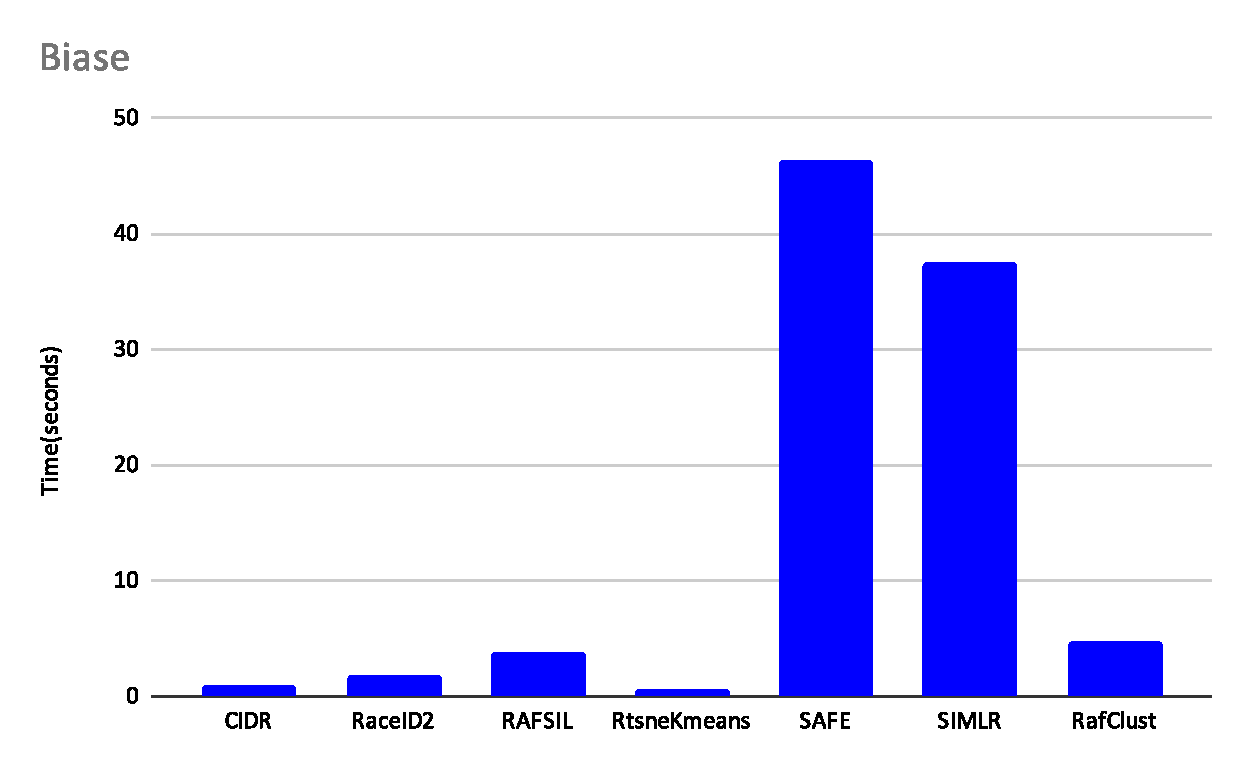
\includegraphics[width = \linewidth]{Biase.pdf}}
      \medskip  
    \end{minipage}
    \begin{minipage}[b]{0.45\linewidth}
      \centering
      \centerline{
        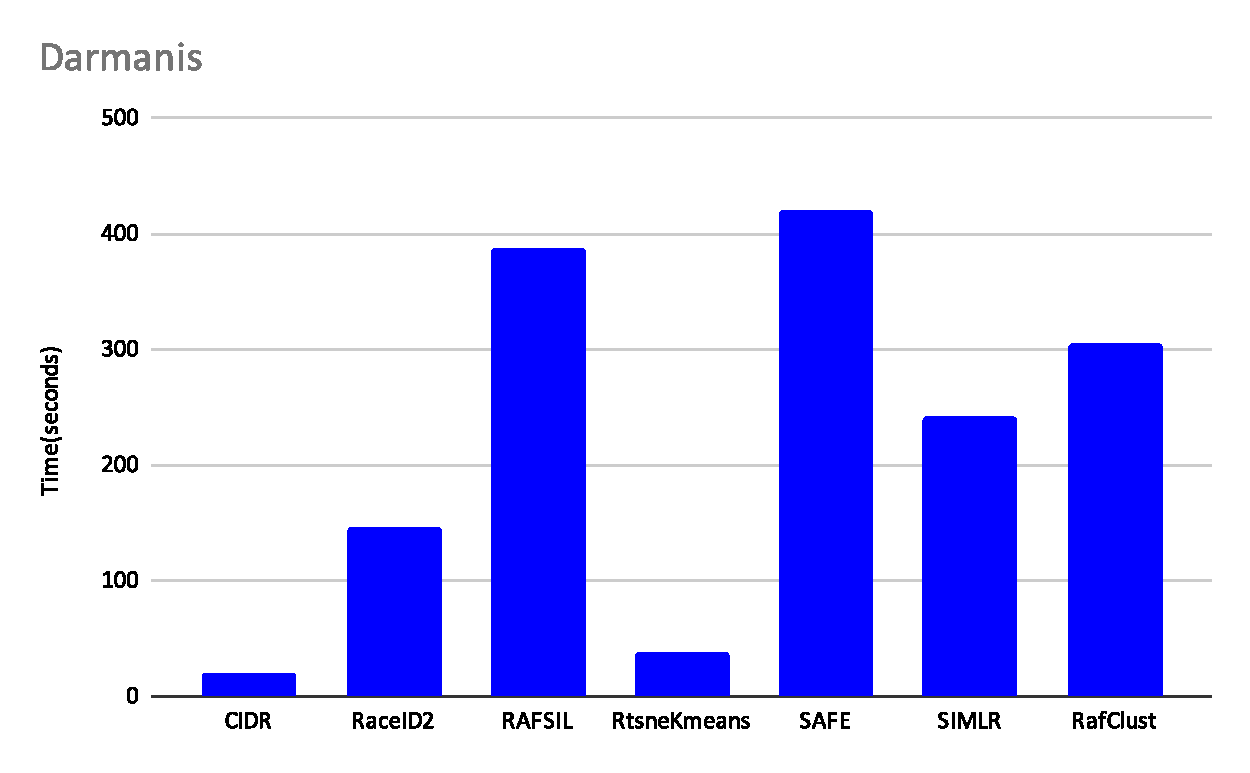
\includegraphics[width =\linewidth]{Darmanis.pdf}}
      \medskip  
    \end{minipage}
      \begin{minipage}[b]{0.45\linewidth}
      \centering
      \centerline{
        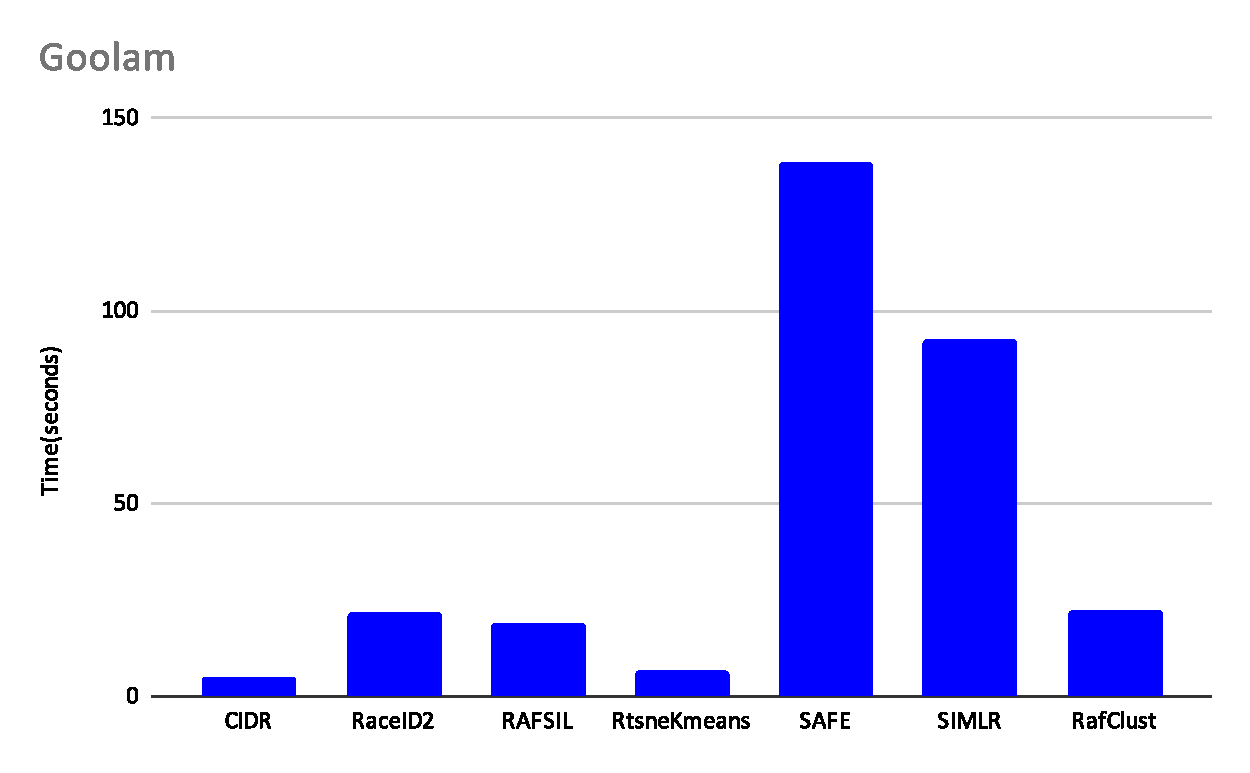
\includegraphics[width = \linewidth]{Goolam.pdf}}
      \medskip  
    \end{minipage}
    \begin{minipage}[b]{0.45\linewidth}
      \centering
      \centerline{
        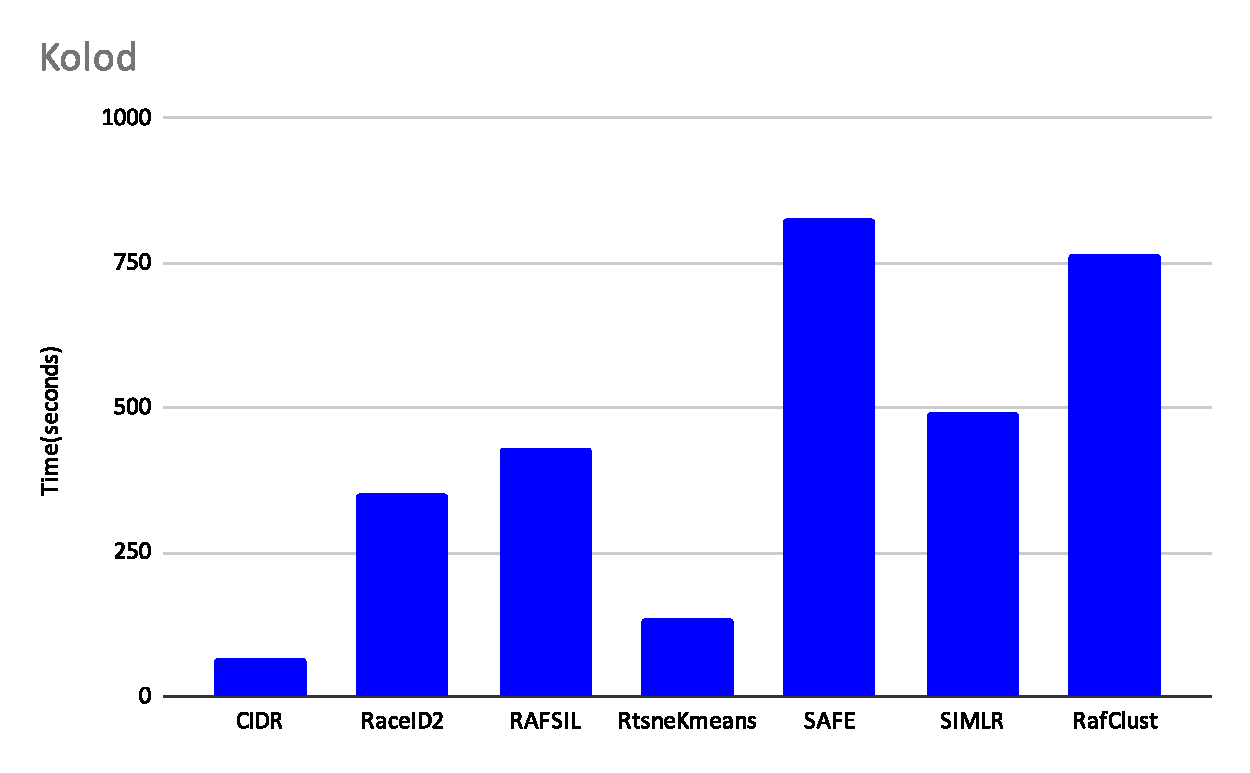
\includegraphics[width =\linewidth]{Kolod.pdf}}
      \medskip  
    \end{minipage}
    \begin{minipage}[b]{0.45\linewidth}
        \centering
        \centerline{
          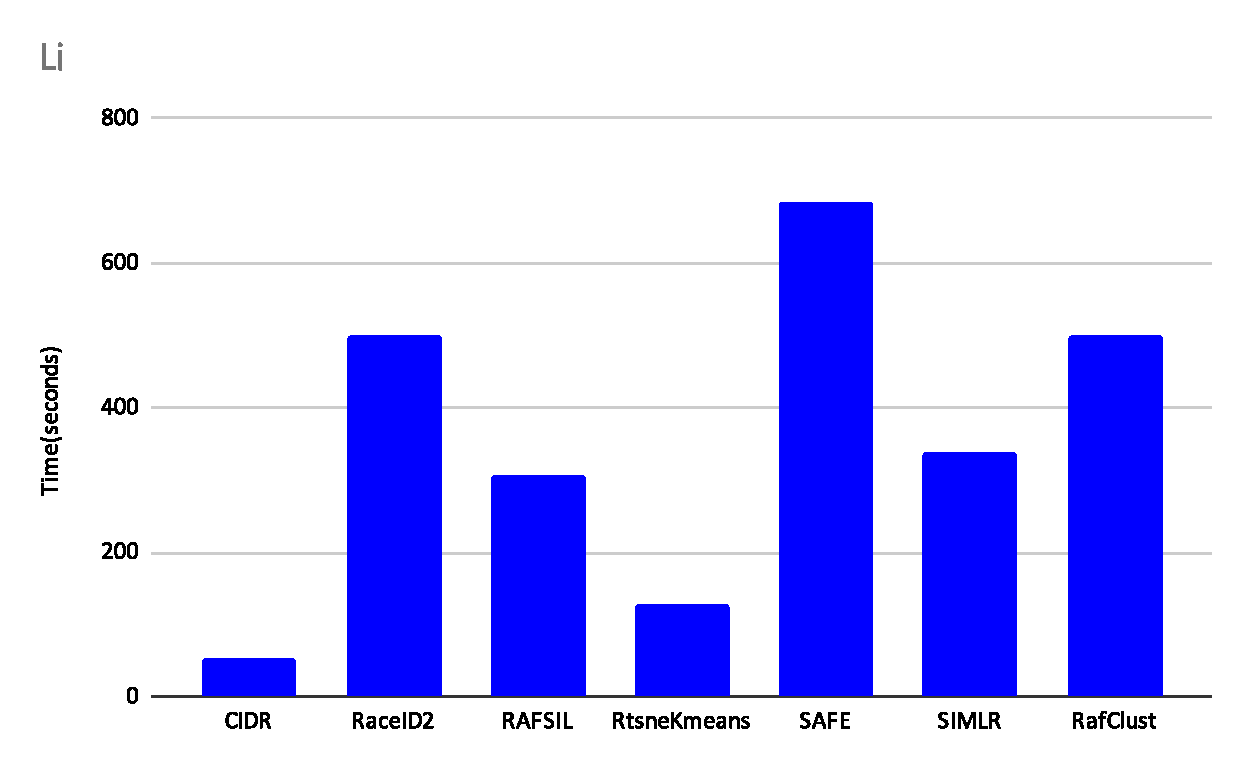
\includegraphics[width =\linewidth]{Li.pdf}}
        \medskip  
      \end{minipage}
      \begin{minipage}[b]{0.45\linewidth}
        \centering
        \centerline{
          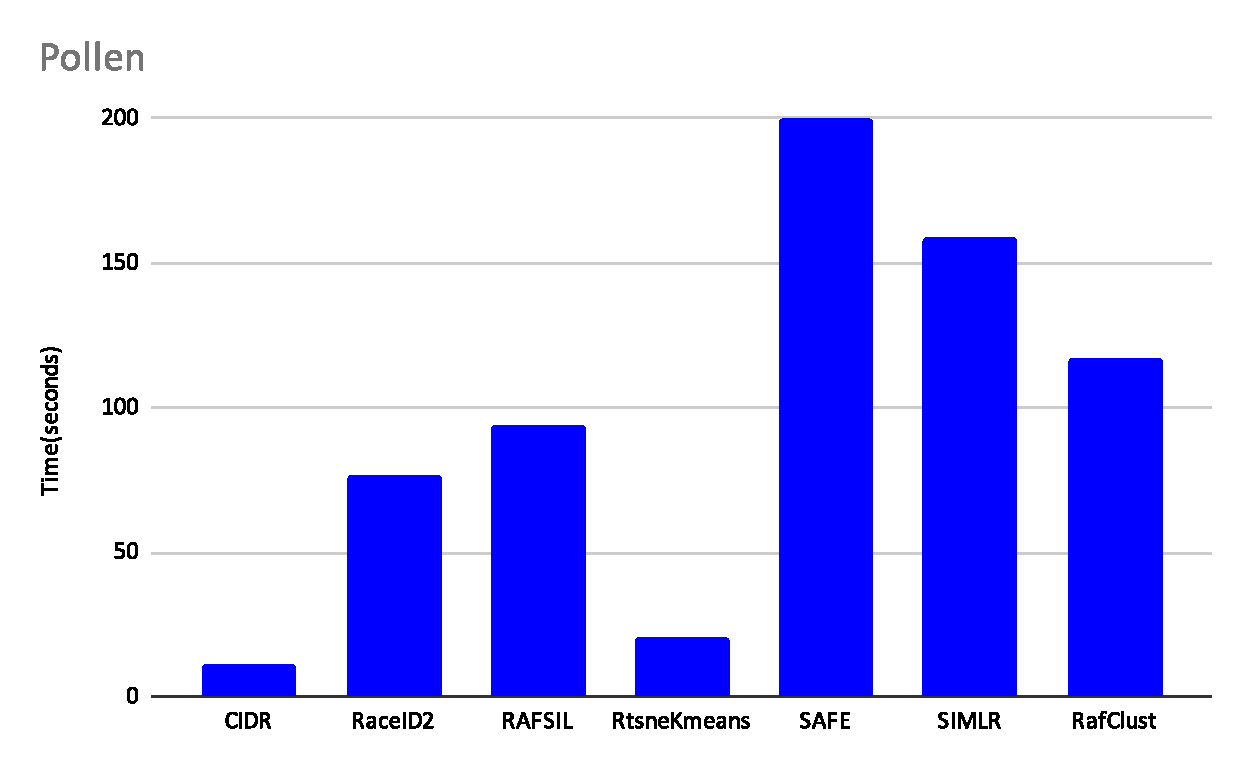
\includegraphics[width =\linewidth]{Pollen.pdf}}
        \medskip  
      \end{minipage}
      \begin{minipage}[b]{0.45\linewidth}
        \centering
        \centerline{
          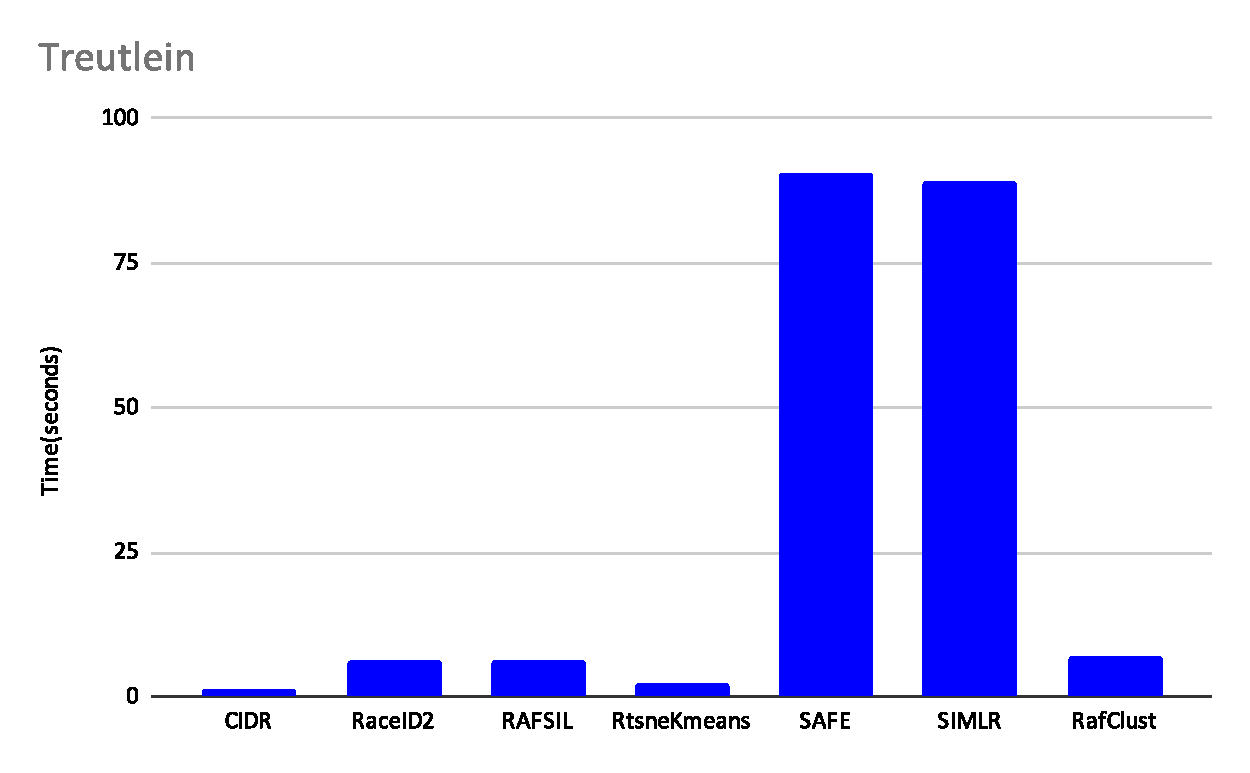
\includegraphics[width =\linewidth]{Treutlein.pdf}}
        \medskip  
      \end{minipage}
      \begin{minipage}[b]{0.45\linewidth}
        \centering
        \centerline{
          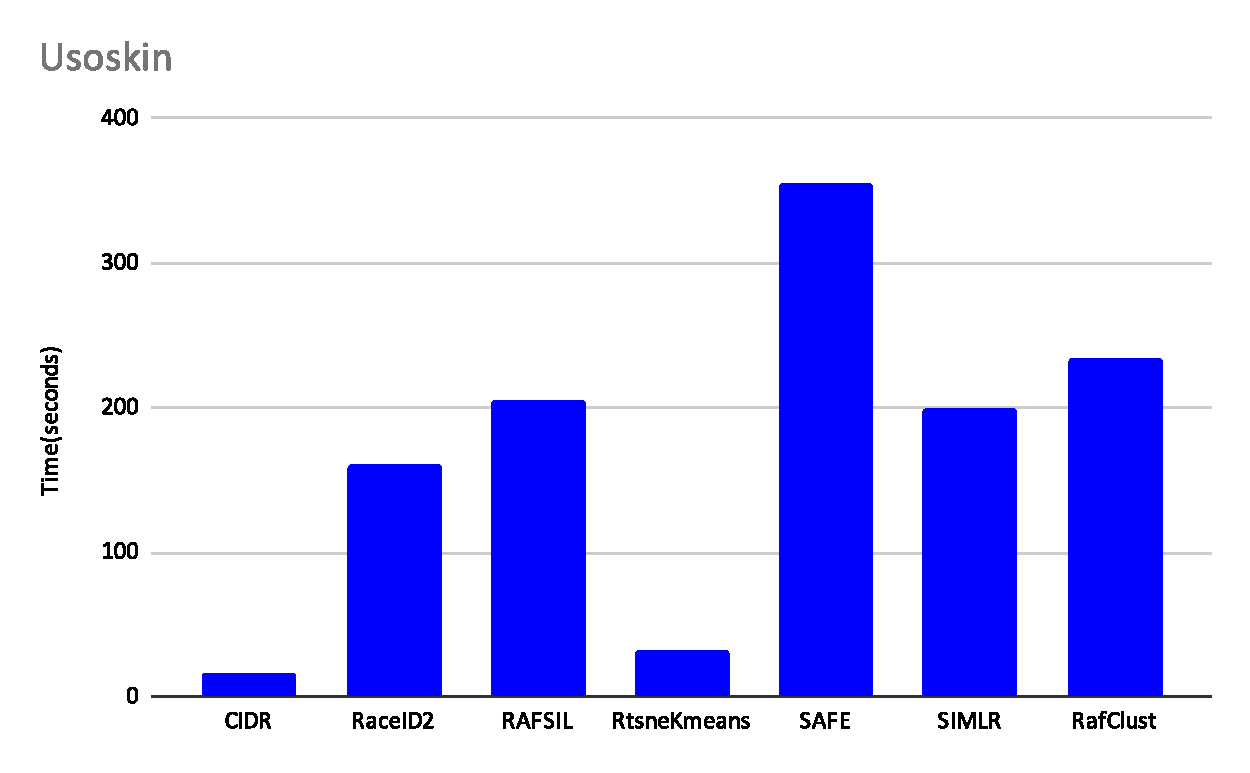
\includegraphics[width =\linewidth]{Usoskin.pdf}}
        \medskip  
      \end{minipage}
      \begin{minipage}[b]{0.45\linewidth}
        \centering
        \centerline{
          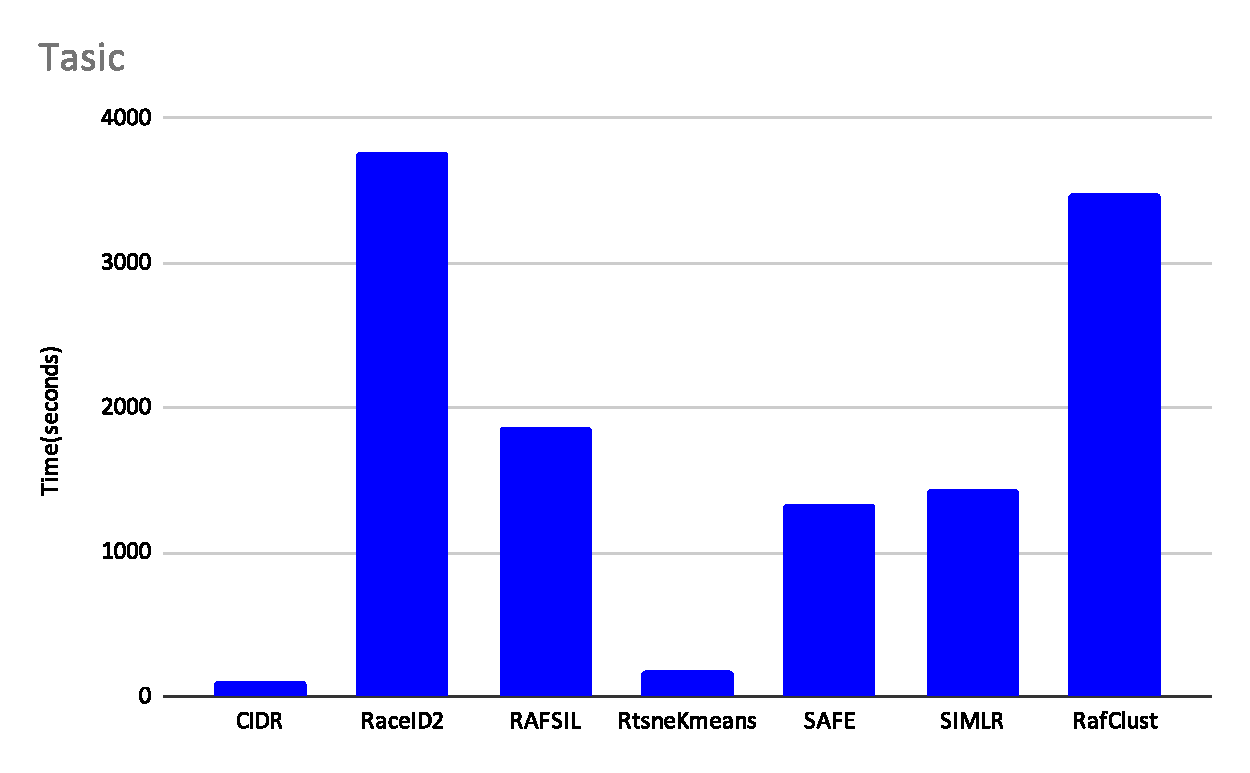
\includegraphics[width =\linewidth]{Tasic.pdf}}
        \medskip  
      \end{minipage}
      \begin{minipage}[b]{0.45\linewidth}
        \centering
        \centerline{
          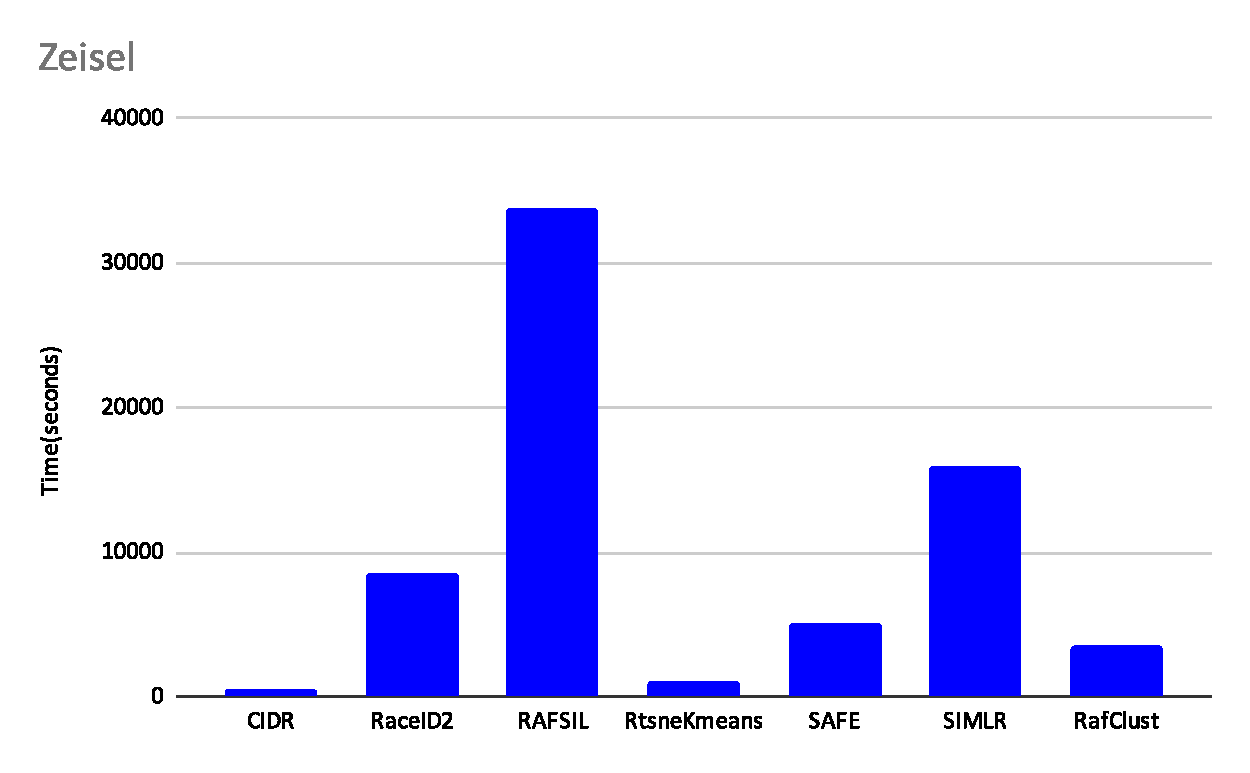
\includegraphics[width =\linewidth]{Zeisel.pdf}}
        \medskip  
      \end{minipage}
    \caption{
    RafClust 与其它六种方法在 10 个数据集上的中位数运行时间示意图。
    }
    \label{fig:running-detail}
    \vspace{-0.5em}
  \end{figure*}
 
  \begin{figure}[!htbp]
    \centering
    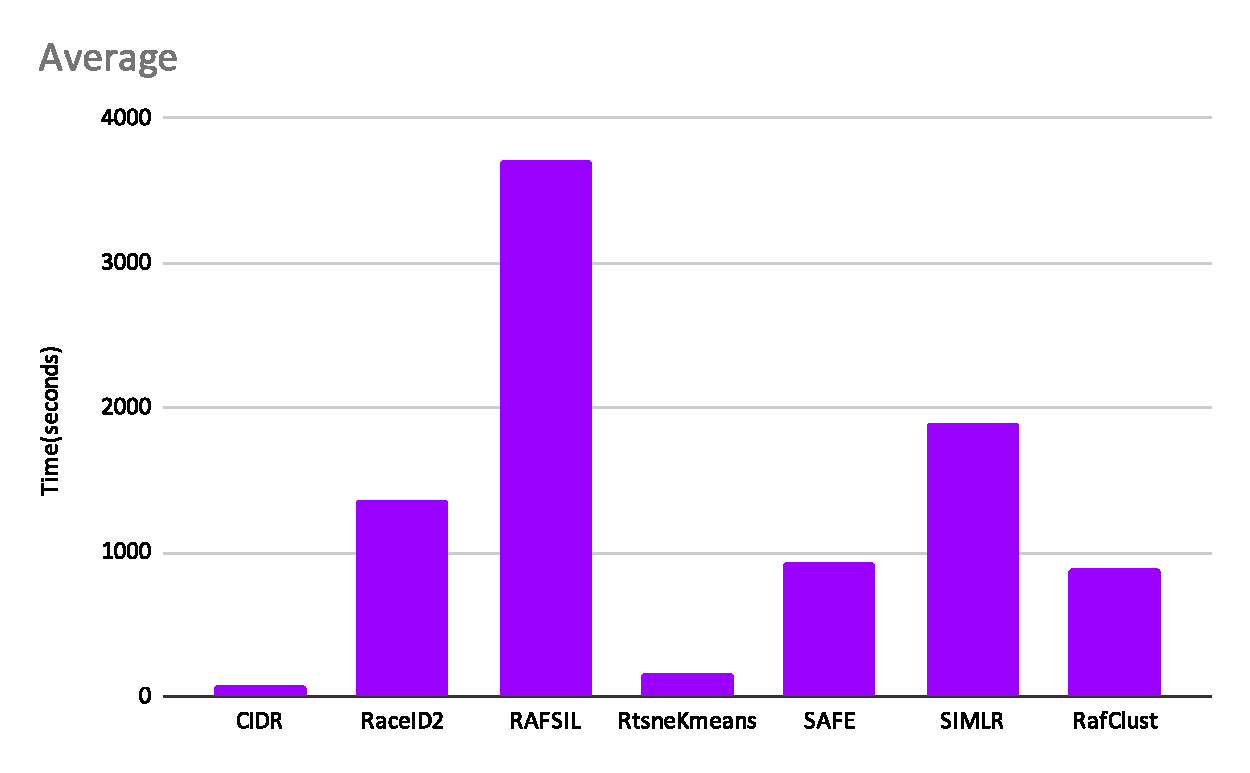
\includegraphics[width=0.9\textwidth]{Average.pdf}
    \caption{
    RafClust 与其它六种方法在 10 个数据集上的中位数运行时间示意图。
    }
    \label{fig:running-summary}
\end{figure}

\begin{figure}[!htbp]
    \centering
    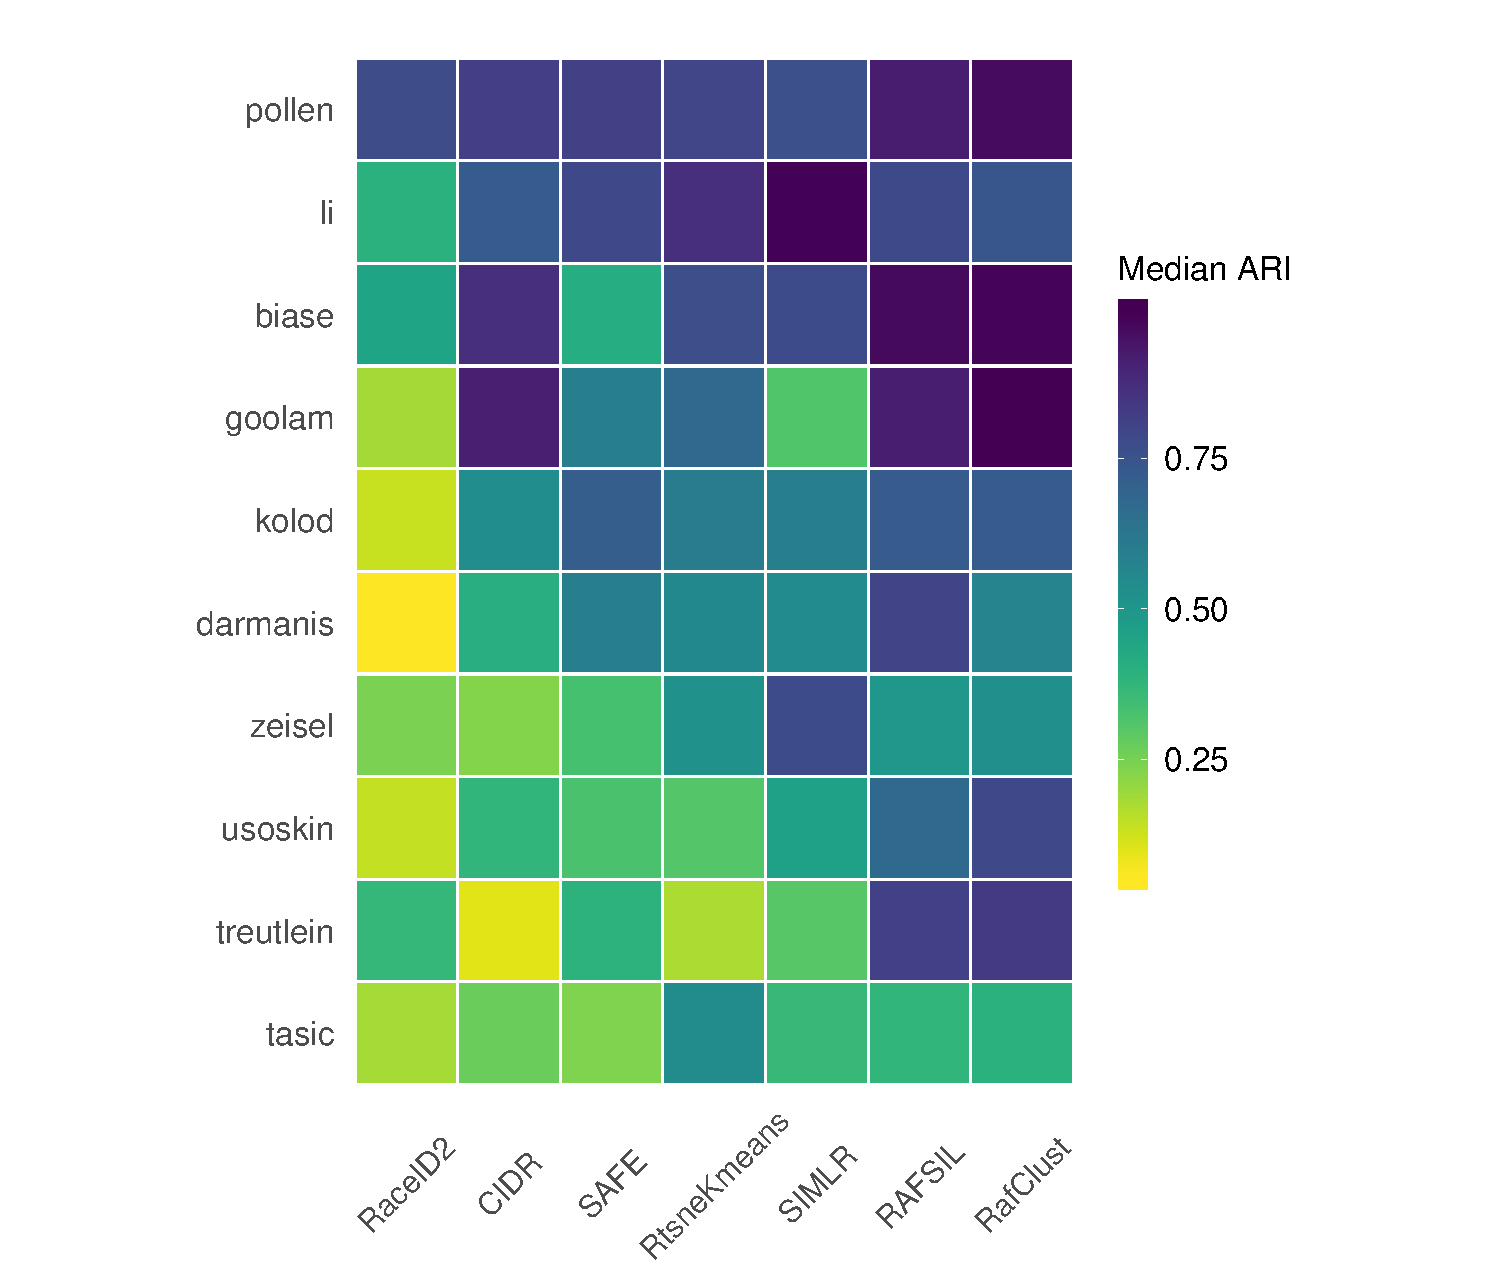
\includegraphics[width=0.9\textwidth]{Figure_ari_summary.pdf}
    \caption{
    % Median ARI across different runs on the same dataset for the methods
    不同数据集上不同方法的 ARI 中位数结果,颜色越深表示 ARI 中位数值越高。
    }
    \label{fig:rafari}
\end{figure}

在这十个数据集上,我们选择了 Goolam 和 Usoskin 两个数据集进行了数据集和聚类结果可视化。
从图 \ref{fig:rafari} 可知 SIMLR、RAFSIL 这两种方法的 ARI 仅次于方法 RafClust,
因此我们选用它们跟 RafClust 对比,在这两个数据集上对聚类结果进行了可视化, 
如图 \ref{fig:goolam-tsne} 和 \ref{fig:usoskin-tsne} 所示。
总体上来看, SIMLR 和 RAFSIL 均比原始数据上直接进行 t-SNE 结果要好,
但是 RafClust 表现比 SIMLR、RAFSIL 这两种方法结果要好。

\begin{figure}[!htbp]
  \centering
  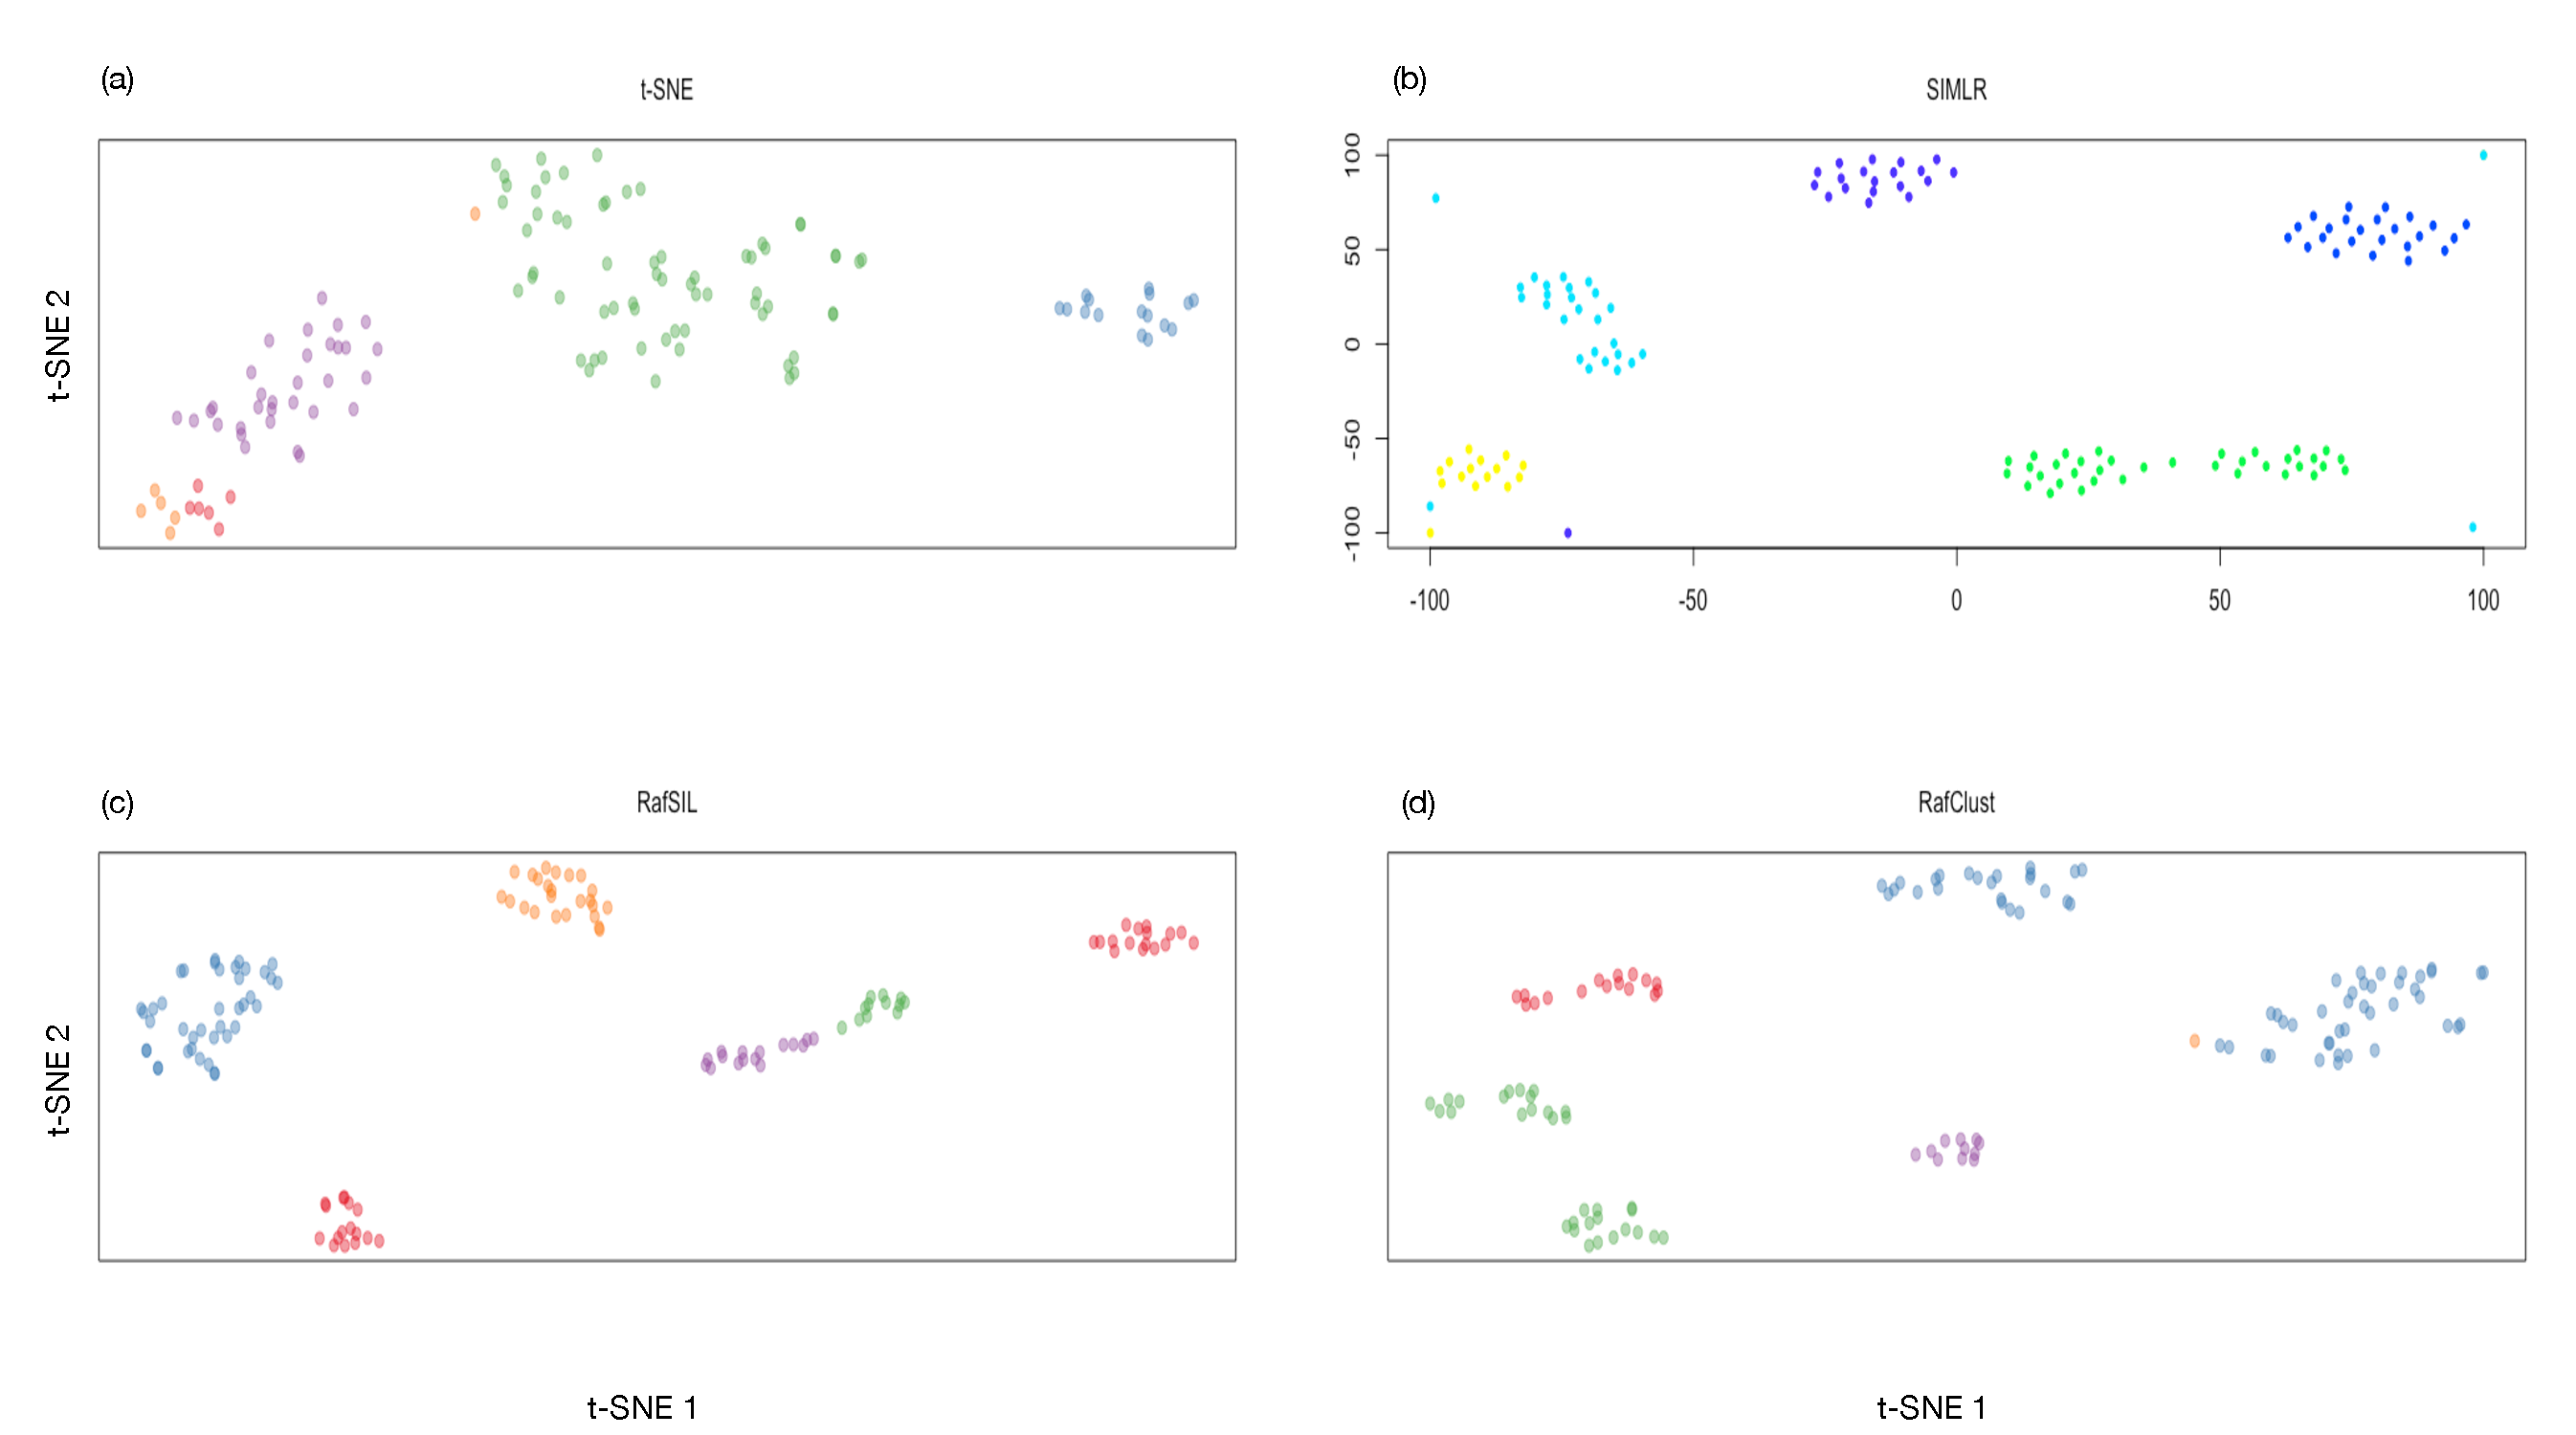
\includegraphics[width=\linewidth]{goolam-tsne.pdf}
  \caption{
  Goolam 数据集上的可视化。
  (a) 原始数据集使用 t-SNE 可视化,使用了真实的细胞类别标签进行着色,参数 perplexity 设置为 20。
  (b)  SIMLR 方法聚类结果可视化。
  (c)  RAFSIL 方法聚类结果可视化,参数 perplexity 设置为 20。
  (d)  RafClust 方法聚类结果可视化,对距离矩阵使用 t-SNE 进行可视化,参数 perplexity 设置为 20。
  }
  \label{fig:goolam-tsne}
\end{figure}


\begin{figure}[!htbp]
  \centering
  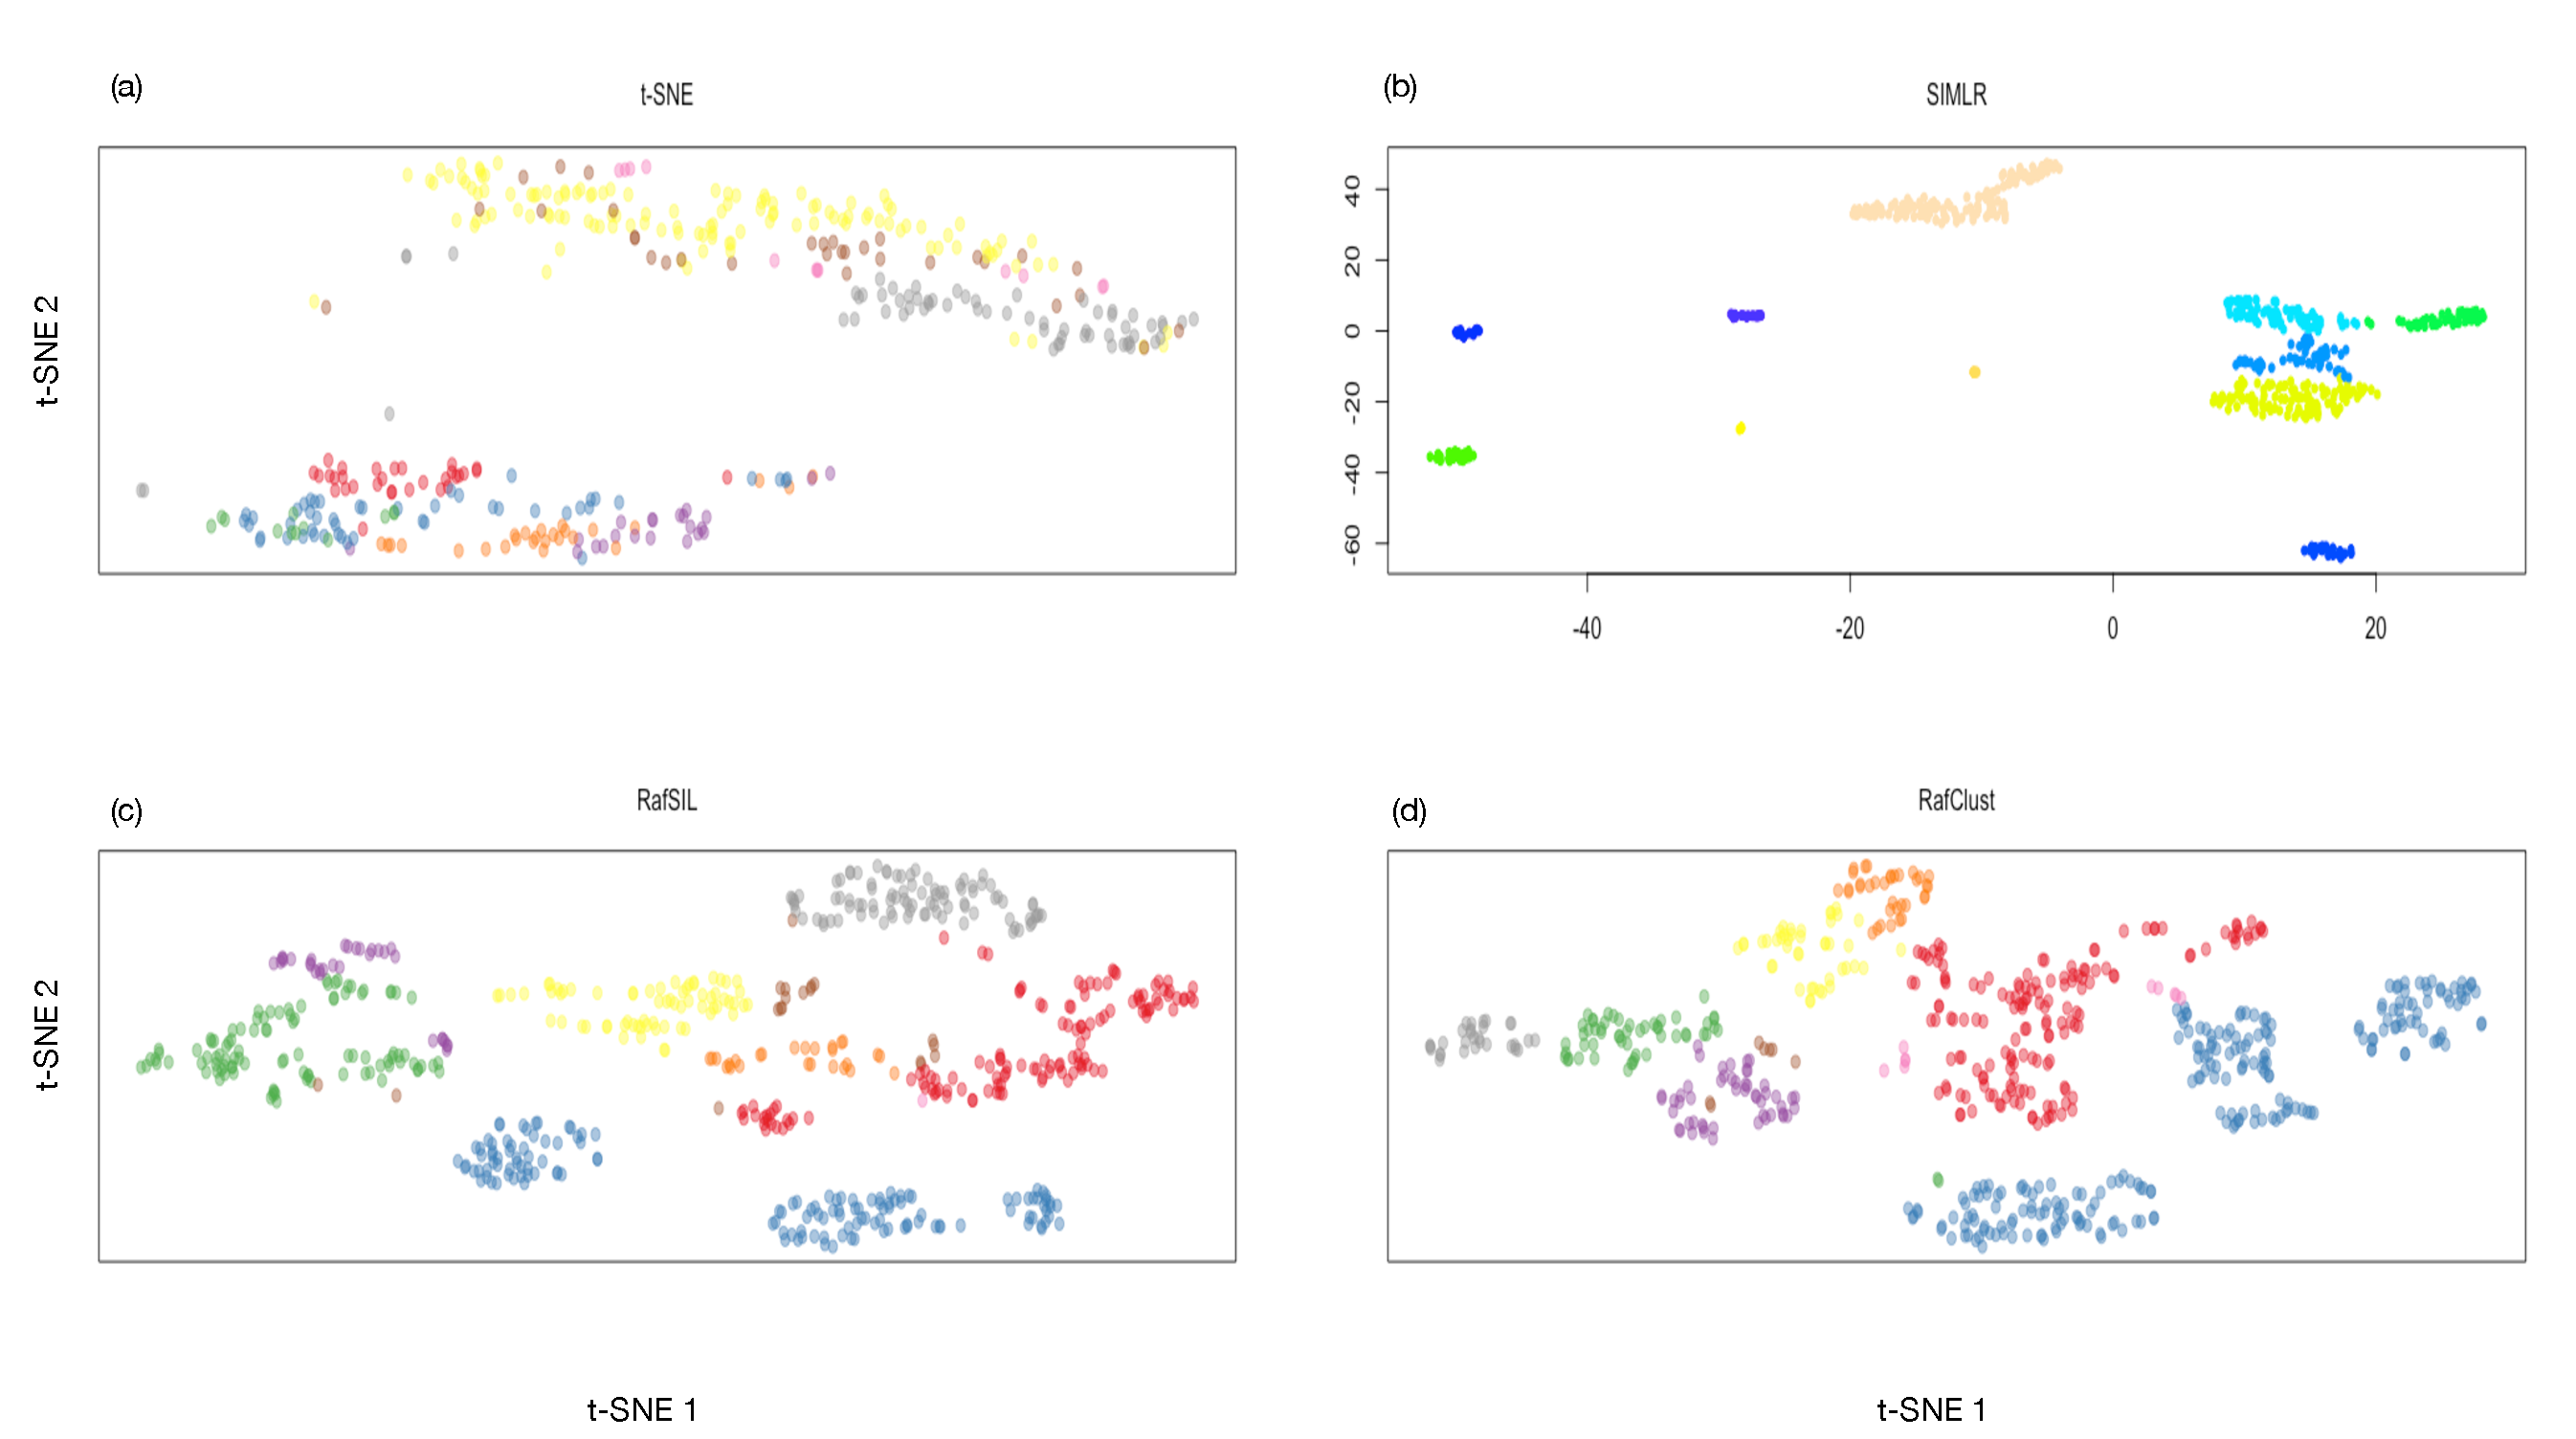
\includegraphics[width=\linewidth]{usoskin-tsne.pdf}
  \caption{
  Usoskin 数据集上的可视化。
  (a) 原始数据集使用 t-SNE 可视化,使用了真实的细胞类别标签进行着色,参数 perplexity 设置为 20。
  (b)  SIMLR 方法聚类结果可视化。
  (c)  RAFSIL 方法聚类结果可视化,参数 perplexity 设置为 20。
  (d)  RafClust 方法聚类结果可视化,对距离矩阵使用 t-SNE 进行可视化,参数 perplexity 设置为 20。
  }
  \label{fig:usoskin-tsne}
\end{figure}


% \subsection{DoRC 方法的实验结果}

% \subsubsection{数据集}
% \label{subsec:datasets} 

% 第一个数据集 \textit{PBMCs\_68k}由 68579 个从健康供体收集的 PBMCs 组成 \cite{zheng2017massively}。
% 11 个纯化的 PBMCs 亚群的单细胞表达谱被用作细胞类型标签的参考。
% 该数据集可在 \url{www.10xgenomics.com} 下载。

%第二个数据集textit{MSE/20k}包含了来自小鼠大脑Arc-ME区域周围的 ${sim} 20$k scRNA-seq图谱 \cite{campbell2017molecular}。
%作者将神经元细胞分为34个簇。
%和非神经元细胞通过二传聚类方法分为30个聚类。
%我们只关注30个非神经元集群,其中包括8092个非神经元细胞。
%数据集 (GSE93374) 是从\url{https://hemberg-lab.github.io/scRNA.seq.datasets/mouse/brain/}下载的。

% 第二个数据集 \textit{Jurkat\_293T} 是由 Jurkat 和 293T 的两个表达谱构建的,同样来自同一研究 \cite{zheng2017massively}。
% Jurkat 数据集由 3258 个细胞组成,而 293T 数据集由 2885 个细胞组成。
% 首先,从 293T 数据集中不放回抽样 1500 个细胞。
% 然后,通过从 Jurkat 数据集中取样不同数量的细胞,
% 产生 8 个数据集,其中 Jurkat 细胞数占比分别为 0.5\%、1\%、1.5\%、2\%、2.5\%、5\%、10\%、15\%。
% 这两个数据集的表达矩阵也可以从 \url{www.10xgenomics.com} 下载。

% 最后一个数据集 \textit{Splatter\_500} 是一个人工仿真 scRNA-seq 数据,
% 通过使用 R 包 Splatter \cite{zappia2017splatter},由 500 个细胞组成。
% 与两种细胞类型: 25 个细胞是罕见的 (也就是 rare cells),其它 475 个细胞是丰富的 (也就是 abundant cells)。
% 在这个数据集中,每个细胞有 5000 个基因。
% 在 R 中我们使用下面的命令来生成这个数据集:

% \texttt{splatSimulate(group.prob = c(0.95, 0.05), method = groups, 
% verbose = F, batchCells = 500, de.prob = c(0.4, 0.4), out.prob = 0, 
% de.facLoc = 0.4, de.facScale = 0.8, nGenes = 5000)}

% \subsubsection{评价指标}

% 在两类实验中,直接构建一个混淆矩阵 (confusion matrix),其数字为真阳性 (TP)、假阳性 (FP)、真阴性 (TP)、假阴性 (FN)。
% 混淆矩阵上的精确率 Precision、召回率 Recall 和综合评价指标 F1-score 可以很容易地计算,如等式 \ref{eq:precision}、\ref{eq:recall}、\ref{eq:f1score} 所示。
% % \begin{equation}
% %     \label{eq:precision}
% %     \text{Precision} = \frac{\text{TP}}{\text{TP} + \text{FP}}
% % \end{equation}
% % \begin{equation}
% %     \label{eq:recall}
% %     \text{Recall} = \frac{\text{TP}}{\text{TP} + \text{FN}}
% % \end{equation}
% \begin{equation}
% \label{eq:f1score}
% \text{F1-score} = 2 \times \frac{\text{Precision} \times \text{Recall}}{ \text{Precision} + \text{Recall}}
% \end{equation}
% 在模拟实验中,对于其 DoRC 分数满足 IQR 阈值的标准的被认定为是稀有细胞。
% 对于实验中采用的 \textit{Jurkat\_293T} 数据集,计算出 Jurkat 细胞的 F1 分数。

% \subsubsection{实验结果分析}
%\subsubsection{DoRC 概览}
%\label{subsec:dorc}


\subsubsection{树突状细胞的异质性分析}

我们将 DoRC 应用于包含 ${\sim}68$k 外周血单核细胞的 scRNA-seq 数据集 (PBMCs) 的标注进行比对。
 \textit{PBMCs\_68k}数据集是知名的包含有 11个 纯化的免疫细胞亚型的数据集,由 68579 个从健康供体收集的 PBMCs 组成 \cite{zheng2017massively},
可在 \url{www.10xgenomics.com} 下载。
研究者首先对细胞进行了无监督聚类,
然后根据之前已知的标记对类进行注释 (图 \ref{supp-fig:dorcsummary} A)。
我们将 DoRC 的分数叠加在这一个二维图上 (图 \ref{supp-fig:dorcsummary} B)。
最高 0.1\% 的 DoRC 分数对应的是最小的, 
清晰地标注了含有巨核细胞的 CD34+ 类别 (图 \ref{fig:dorcsummary} A)。
据报道,巨核细胞只含有整个细胞集的 0.3\% \cite{zheng2017massively}。
然后,我们将这一比例从 0.1\% 增加到 1.0\%,随后又增加到 3.0\%,
然后下一批次的细胞亚型被选入扩展的稀有细胞集合中。
这些细胞包括单核细胞和树突状细胞亚型的亚类 (图 \ref{fig:dorcsummary} B-C)。
这个案例研究展示了 DoRC 在检测不同比例的稀有细胞方面的表现。

\begin{figure*}[!htbp]
    \centering
    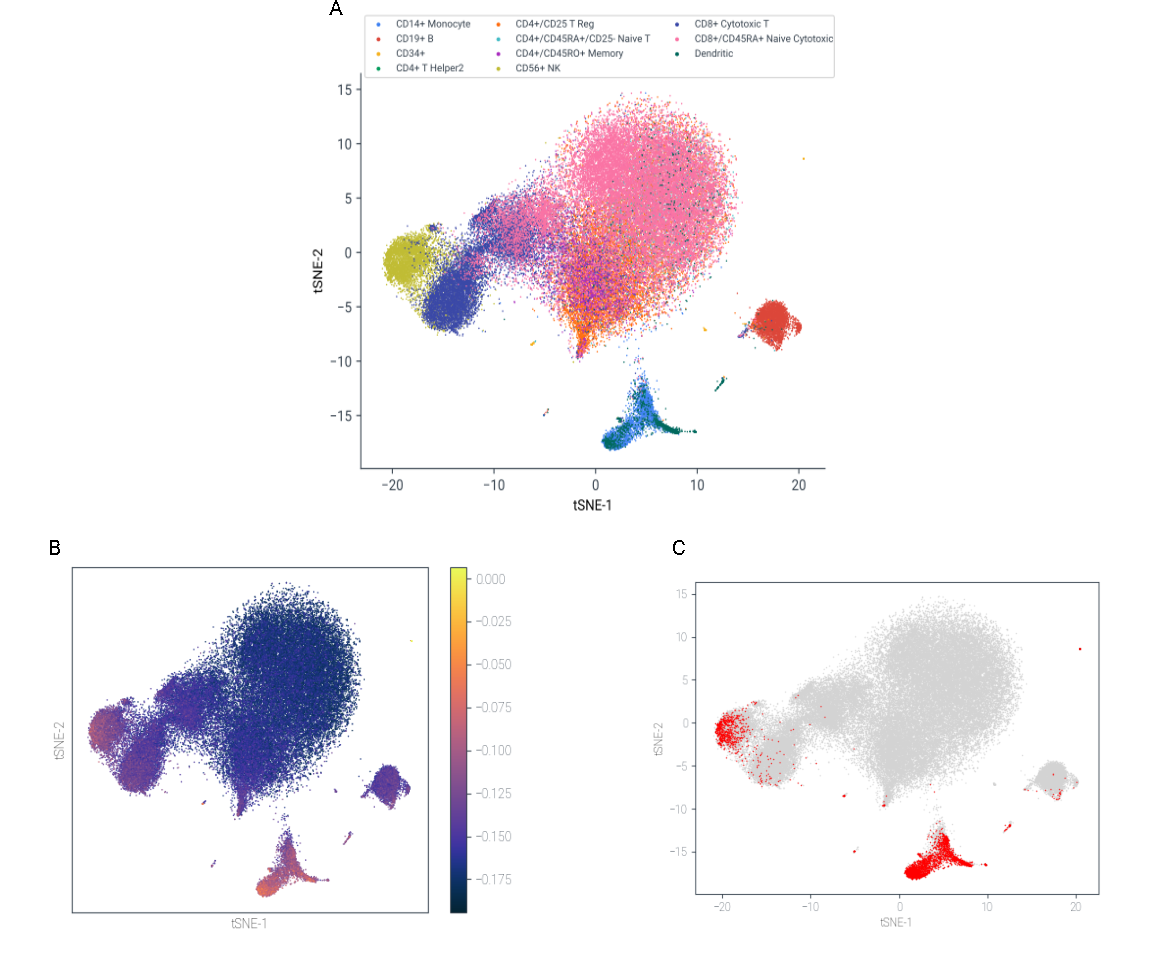
\includegraphics[width=0.9\textwidth]{DoRCSummarySI.pdf}
    \caption{
    % Performance evaluation of DoRC on PBMCs\_68k. 
    % (A) t-SNE based 2D embedding of the data with color-marked cluster identities as reported by Zheng et al. \cite{zheng2017massively}. 
    % (B) Heat map of DoRC scores for the cells on PBMCs\_68k. 
    % The cluster of megakaryocytes (0.3\%), the rarest of all the cell types are assigned the
    % highest DoRC scores.
    % (C) Rare cells identified by DoRC using IQR-thresholding-criteria
    DoRC 在 PBMCs\_68k 上的性能评估。
    (A) 基于 t-SNE 的二维嵌入数据集可视化图,按 Zheng 等所报道的鉴定的不同类别用不同的颜色标记。
    (B) PBMCs\_68k 上细胞的 DoRC 得分热图。巨核细胞群 (0.3\%),是所有细胞类型中最稀有的细胞,获得了最高的 DoRC 分数。
    (C) 使用 IQR 阈值标准后 DoRC 识别的稀有细胞。
    }
    \label{supp-fig:dorcsummary}
\end{figure*}

\begin{figure*}[!htbp]
    \centering
    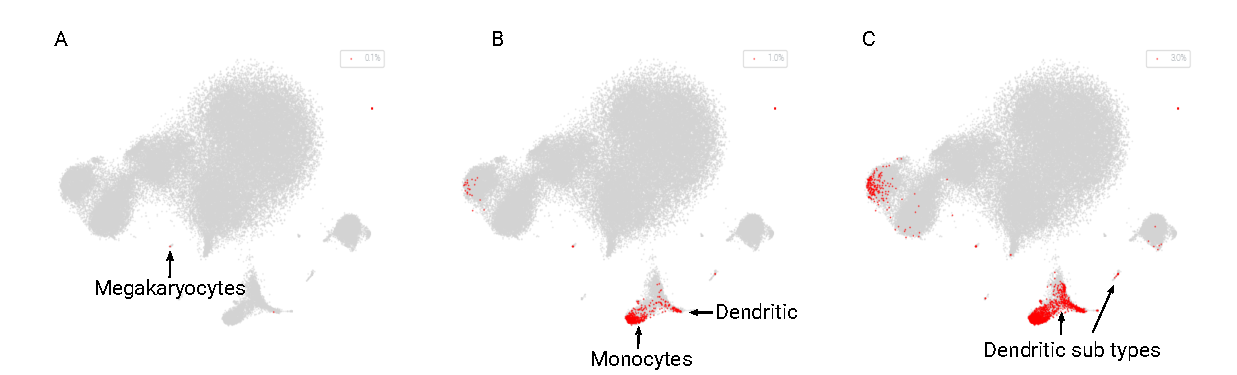
\includegraphics[width=0.9\textwidth]{DoRCSummary.pdf}
    \caption{
    % DoRC discovers cells with varying degrees of rarity. In the ${\sim}68$k PBMC data \cite{zheng2017massively}, minor cell populations with different grades of rarity show up with an
    % increase in the number of selected rare cells. (A-C) The top 0.1, 1.0 and 3.0\% cells, respectively, selected on the basis of DoRC scores are highlighted
    DoRC 发现了不同稀有度的细胞。在 ${\sim}68$k PBMC 数据 \cite{zheng2017massively} 中,不同级别的稀有度对应了一个数量不断增加的稀有细胞群。
    (A-C) 根据 DoRC 得分选出的前 0.1\%、1.0\% 和 3.0\% 的细胞分别以高亮显示。    
    }
    \label{fig:dorcsummary}
\end{figure*}

虽然连续的分数是有意义的,
如果能对细胞稀有性给出二元标注 (binary annotations),则有助于简化后续分析。
为了解决这个问题,本文引入了一个基于得分分布特性的阈值方法。
图 \ref{supp-fig:dorcsummary} C 显示了 ${\sim}68$k PBMC 数据中检测到的细胞。
我们利用基于阈值的二分法来标注稀有细胞,
如预期的那样,
大部分检测到的稀有细胞来源于已知的次要细胞类型,包括巨核细胞、树状细胞和单核细胞,
如图 \ref{supp-fig:dorcsummary} A 上所示的分别对应于 CD34+、树枝状和 CD14+ 单核细胞。


树突状细胞 (DC) 在感知、吞噬和和抗原监视 \cite{villani2017single} 方面起着至关重要的作用。
DCs 是最罕见的免疫细胞类型之一,在 PBMCs \cite{zheng2017massively} 数据集上占比约 0.5\%。
Villani \cite{villani2017single} 的研究划分了六种不同的树突状细胞的亚型。
他们通过荧光激活细胞分选 (FACS) 来分析了树突状细胞、分型 DCs 和单核细胞的表达。
他们在研究中报告的 DC 亚型如下:
$\text{CD141}^+$ DCs (DC1), 
$\text{CD1C}^+${\_}A 常规 DCs (DC2),
$\text{CD1C}^+${\_}B 常规 DCs (DC3),
$\text{CD1C}^-\text{CD141}^-$(DC4), DC5 和浆细胞 DCs (DC6,pDCs)。

我们很好奇树突状细胞亚型是否可以在 PBMCs 数据中被准确识别。
首先,我们在 ${\sim}68$k PBMCs 数据集上应用 DoRC。
DoRC 通过使用基于 IQR 的二分法,共发现了 3844 个稀有细胞。
然后通过 RafClust 对稀有细胞进行聚类 (见 \ref{subsec:rafclust}),得到 12 个子类别。
在这 12 个可区分的聚类中 (C0-C11),
C4、C5、C9 和 C11 完全由树枝状细胞组成,根据 Zheng 等人提供 \cite{zheng2017massively}的标注,
如图 \ref{fig:dorc_dendritic} A-C 所示。
对于这 4 个 DC 类别,我们进行差异表达分析,找出细胞类型特异性基因 (见 \ref{subsec:de})。
共有 21 个基因被检测为细胞类型特异性基因,使用阈值为 log2(1.5) 的 FC (fold change)。
通过将我们的差异基因与 Villani \cite{villani2017single} 报道的基因进行叠加。
我们可以有信心地解析 6 个亚型中的 5 个 (DC1、DC2、DC4、DC6) (图 \ref{fig:dorc_dendritic} D、表 \ref{supp-tbl:dendritic})。
从 \cite{villani2017single} 可以看出, DC5 是未识别的 (unresolved) 的,因为该类型是新分离出来的罕见类型。
在 t-SNE 二维嵌入图中, DC3 与 DC2 属于同一类 \cite{maaten2008visualizing}。
在 DoRC 检测到的稀有细胞上使用 RafClust 进行聚类,不能完全划分出树突状细胞亚型正确的数量。
然而,在最初 \cite{zheng2017massively}的研究中, DC1 和 DC4 也没有被聚类算法识别到。
事实上,在原始文献 \cite{zheng2017massively} 实验结果的 t-SNE 图上,
这些细胞类型在视觉上共同聚集在自身或单核细胞内。
\begin{figure}[!htbp]
    \centering
    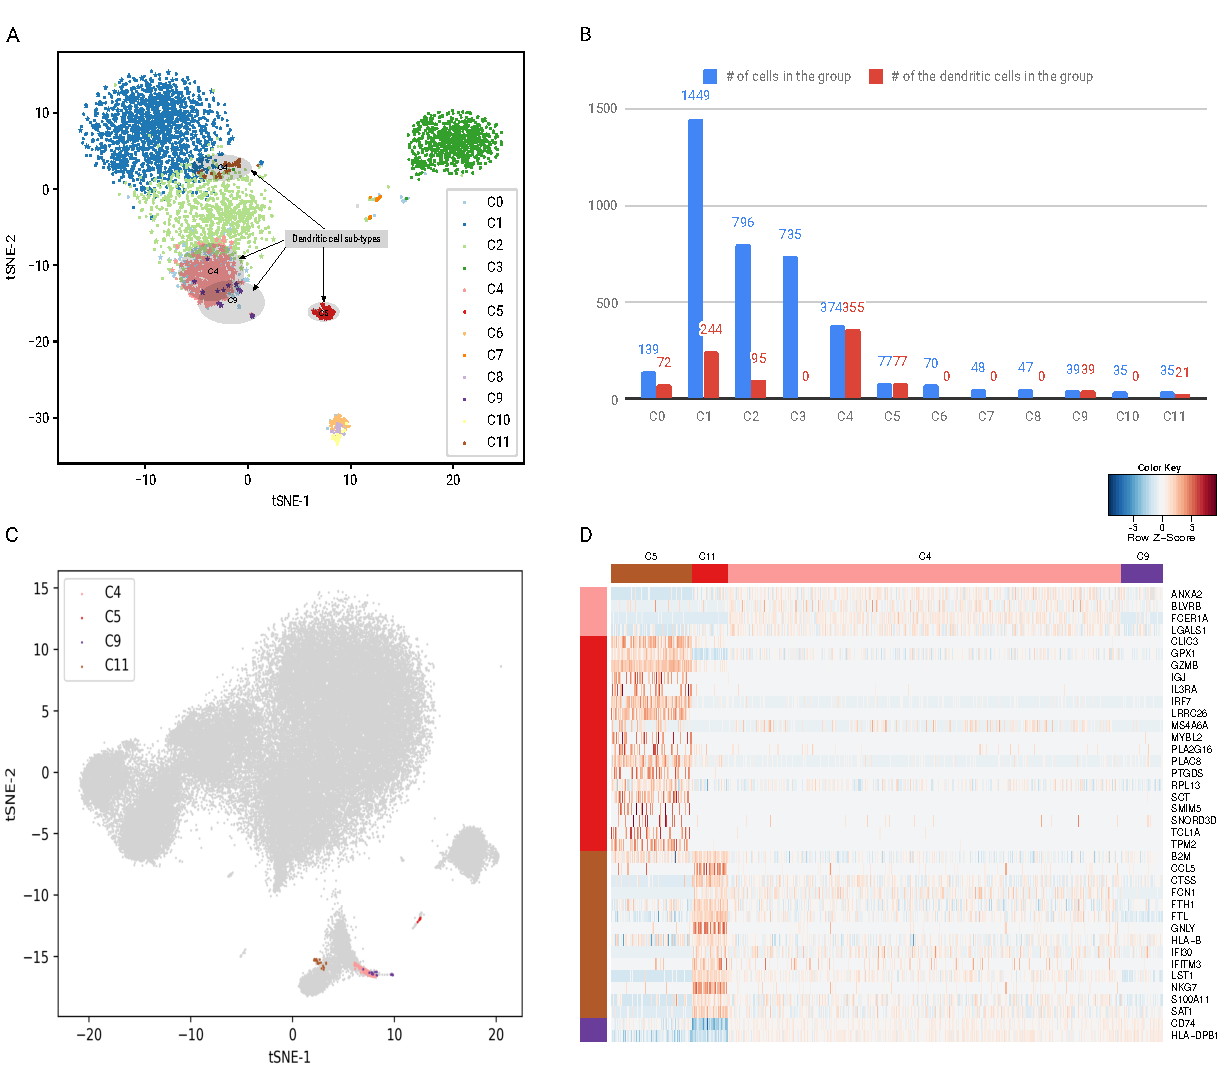
\includegraphics[width=0.9\textwidth]{plot_tsne_dorc_rare_summary.pdf}
    \caption{
    % Human blood dendritic cell heterogeneity delineated by DoRC. 
    % (A) DoRC detected rare cells are clustering into 12 sub types with RafClust, 
    % i.e. C0 (a singleton class), C1, $\ldots$, C11.
    % With the annotation given by \cite{zheng2017massively}, C4, C5, C9, C11 are mostly dendritic cells sub types.
    % Dots with the same color represent one subpopulation by clustering the rare cells with RafClust.
    % For each subpopulation, the cells annotated with asterisks marking are also dendrotic cells according to the annotation given by \cite{zheng2017massively}. 
    % (B) The cells number for each subpopulation and the number of dendrotic cells in this group. 
    % Apparently, dendritic cells hold the majority of the subpopulation in C4, C5, C9, C11.
    % (C) These four dendritic sub-types cells are highlighted on the \textit{PBMCs\_68k} dataset t-SNE-based 2D plot.
    % (D) Characterization of dendritic cell sub-types utilizing markers obtained from DE analysis (See \ref{subsec:de})
    DoRC 检测到人类血液树突状稀有细胞的异质性。
    % (A) DoRC 检测到的稀有细胞在 RafClust 中被聚成 12 个亚型,即 C0,C1,$\ldots$,C11。
    % 通过 \cite{zheng2017massively} 给出的标注, C4、C5、C9、C11 多为树枝状细胞亚型。
    % 用 RafClust 聚类稀有细胞,同种颜色的点代表一个亚群。
    % 对于每个亚群,根据 \cite{zheng2017massively} 给出的注释,
    % 用星号标记的细胞也是树突状细胞。
    % (B) 每个亚群的细胞数和本组中树突状细胞的数量。
    % 显然,树枝状细胞在 C4、C5、C9、C11 的亚群中占有多数。
    % (C) 这四种树枝状亚型细胞在 \textit{PBMCs\_68k} 数据集的 t-SNE 二维图上突出显示。
    % (D) 利用从 DE 分析中获得的标记来描述树突状细胞亚型的特征 (见节 \ref{subsec:de})
    }
    \label{fig:dorc_dendritic}
\end{figure}

\begin{table}[!htbp]
    \centering
    \caption{
        %The dendritic cell types correspond to class types reported by Villani \cite{villani2017single}
        树枝状细胞类型对应于 Villani 报告的细胞类别 \cite{villani2017single}
        }
    \label{supp-tbl:dendritic}
    \resizebox{\columnwidth}{!}{
    \begin{tabular}{clc}
    \hline
    Class type & \multicolumn{1}{c}{Marker gene(s)}                                                                                                                                   & Corresponding class type \\ \hline
    C4         & ANXA2, BLVRB, \textbf{FCER1A}, LGALS1	                                                                                                                                         & DC2                      \\ \hline
    C5         & \begin{tabular}[c]{@{}l@{}}CLIC3, GPX1, \textbf{GZMB}, \textbf{IGJ}, \textbf{IL3RA}, \textbf{IRF7}, LRRC26, MS4A6A, MYBL2,\\ PLA2G16, PLAC8, PTGDS, RPL13, SCT, SMIM5, SNORD3D, TCL1A, TPM2\end{tabular} & DC6                      \\ \hline
    C9         & \begin{tabular}[c]{@{}l@{}}B2M, CCL5, CTSS, FCN1, FTH1, \textbf{FTL}, GNLY, HLA-B, IFI30, \textbf{IFITM3}, \textbf{LST1},\\ NKG7, S100A11, SAT1\end{tabular}                                    & DC4                      \\ \hline
    C11        & CD74, \textbf{HLA-DPB1}                                                                                                                                                       & DC1                      \\ \hline
    \end{tabular}
    }

    \begin{tablenotes}
        \small
        %\item Note: Those genes marked in bold are acting as  marker genes in the corresponding class type.
        \item 注: 用粗体标记的基因在相应的类型中起着标志 (Marker) 基因的作用。
      \end{tablenotes}

\end{table}

\subsubsection{人工伪造的稀有细胞识别}
\label{subsec:recplanted} 


本文设计了一个在模拟数据集 Jurkat\_293T 上的实验来评估 DoRC 在细胞类型识别上的性能表现。
 \textit{Jurkat\_293T} 是由 Jurkat 和 293T 的两个表达谱构建的,同样来自同一研究 \cite{zheng2017massively}。
Jurkat 数据集由 3258 个细胞组成,而 293T 数据集由 2885 个细胞组成。
首先,从 293T 数据集中不放回抽样 1500 个细胞。
然后,通过从 Jurkat 数据集中取样不同数量的细胞,
产生 8 个数据集,其中 Jurkat 细胞数占比分别为 0.5\%、1\%、1.5\%、2\%、2.5\%、5\%、10\%、15\%。
这两个数据集的表达矩阵也可以从 \url{www.10xgenomics.com} 下载。
作者利用每个细胞的单核苷酸变异 (SNV) 谱来确定其系谱。
我们认为这种基于基因型的标注接近真实的细胞标签。

对于每个数据集, F1-score 是用通过 DoRC 评分和 IQR 阈值标准确定预测标签,然后与两个类的真实标签进行计算。
重复这个过程 100 次,可以得到该数据集的 F1 分数的标准差。
标准差反应了该方法识别人工伪造的稀有细胞的稳定性 (图 \ref{fig:jurkat} A)。 
F1-score 反应了精度和灵敏度之间的平衡。
当稀有率处于低水平时,即 0.5\% 和 1\% 时, DoRC 无法匹配 FiRE。
但是,当稀有率从 1.5\% 增加到 15\% 时, DoRC 的性能优于 FiRE。
此外, FiRE 的性能在 15\% 的稀有率下急剧下降,但是 DoRC 更保守,性能损失较小。

特别地,在上述 8 个数据集中,我们选取了稀有细胞占比为 2.5\% 时的对应的数据集作为基准数据集。
%从 100 个生成的数据集中随机选取了一个有 1539 个细胞的混合数据集,作为基准数据集。
从 t-SNE 图 \ref{fig:jurkat} B 上可知,该数据集上 39 个稀有细胞和 1500 个丰富细胞非常清晰地聚成两组。
在 FiRE 和 DoRC 这两种方法中,稀有细胞的得分都清晰地高于丰富细胞类型 (图 \ref{fig:jurkat} C-D)。
每种方法都得到了二元标签 (图 \ref{fig:jurkat} E-F), DoRC 的表现优于 FiRE,
因为它有更好的能力来检测更多的稀有细胞 (图 \ref{fig:jurkat} G-H)。

\begin{figure}[!htbp]
    \centering
    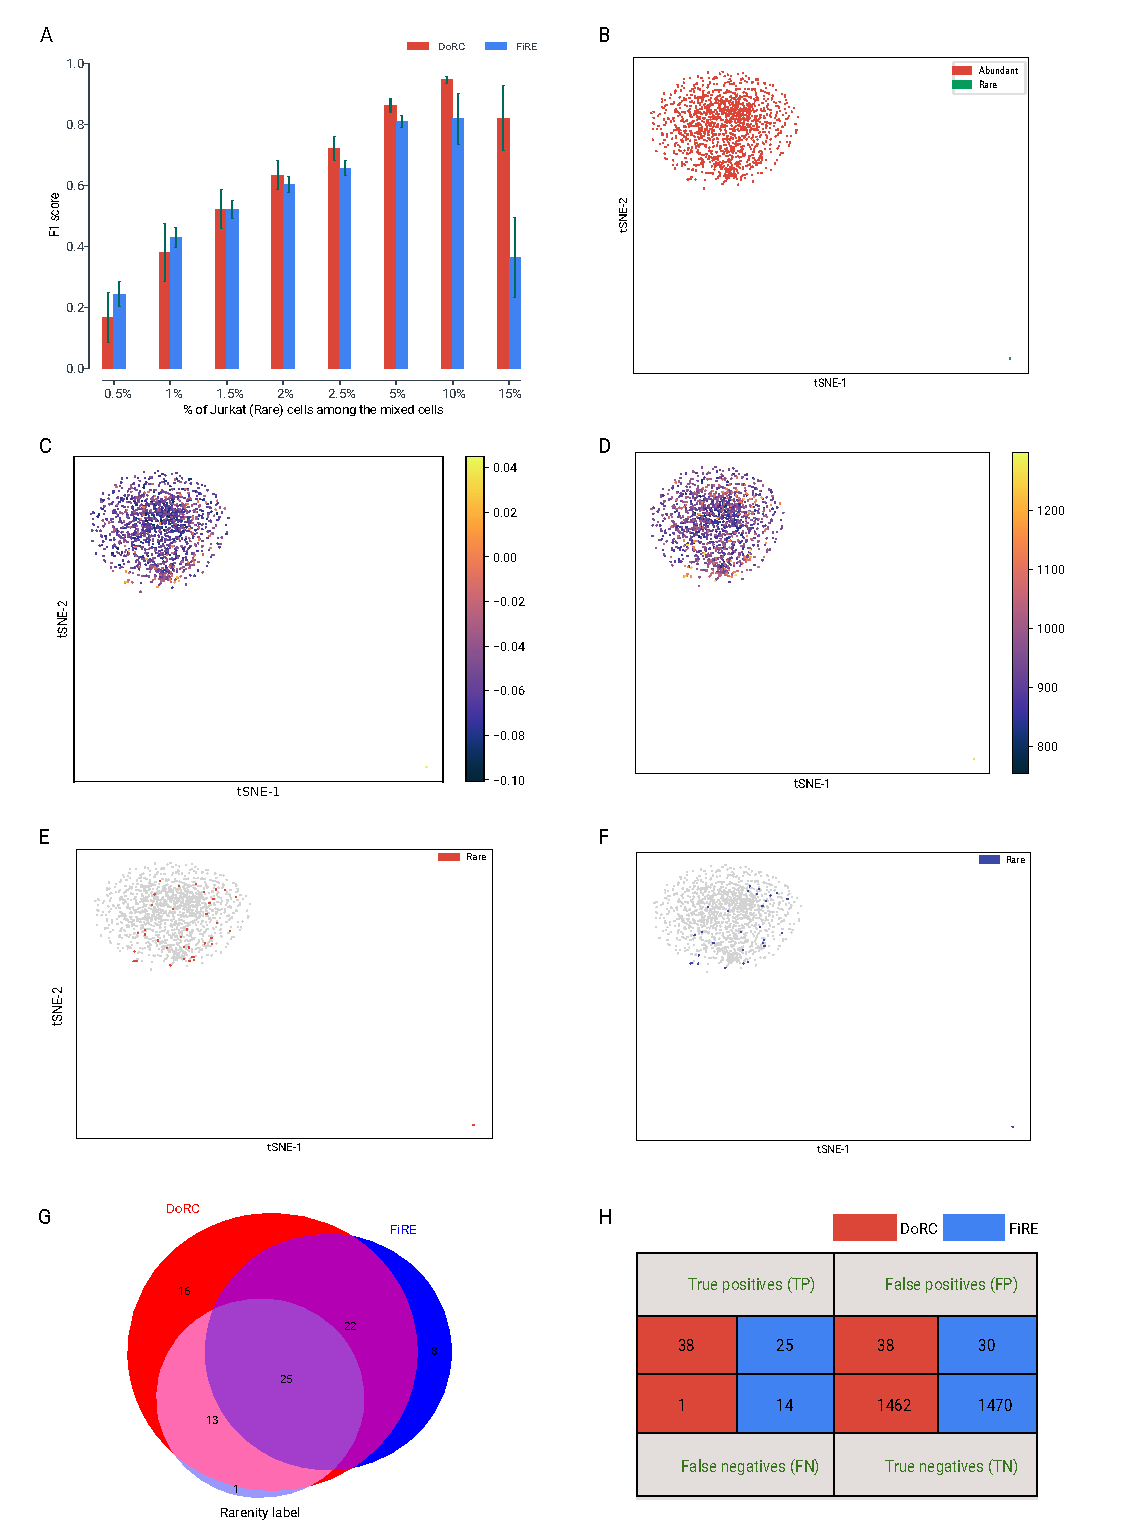
\includegraphics[width=0.9\textwidth]{plot_venn_dorcfire_39summary_compressed.pdf}
    \caption{
    % Detectability of minor cell types in a simulated dataset consisting of Jurkat and 293T cells. 
    % (A) The F1-scores are calculated w.r.t. the rare (Jurkat) population for DoRC and FiRE, 
    % while bioinformatically varying the proportion of artificially planted rare cells.
    % (B) The t-SNE-based 2D embedding of the cells with color-coded identities of the benchmark dataset.
    % (C-D) DoRC and FiRE score intensities plotted on the t-SNE-based 2D map, respectively. 
    % (E-F) The rare cells detected by DoRC and FiRE, respectively, are highlighted.
    % (G) DoRC, FiRE detected rare cells and true rare cells overlap with each other, shown in this Venn diagram. 
    % (H) Detail of the confusion matrices with TP, FP, FN, TN prediction metrics for DoRC and FiRE.
    在由 Jurkat 和 293T 细胞组成的模拟数据集中,次要细胞类型的可检测性示意图。
    % (A) 按照生物信息上逐渐改变人工植入的稀有细胞的比例,计算关于稀有类别 (也就是 Jurkat) 的 DoRC 和 FiRE 的 F1 分数。
    % (B) 基准数据集上细胞的基于 t-SNE 的二维嵌入可视化图,不同颜色代表不同的细胞类别。
    % (C-D) DoRC 和 FiRE 得分分别绘制在基于 t-SNE 的二维嵌入可视化图上。
    % (E-F) DoRC 和 FiRE 分别检测到的稀有细胞,用高亮来显示。
    % (G) DoRC 和 FiRE 检测到的稀有细胞和真正的稀有细胞相互重叠,在该维恩图中显示出来。
    % (H) DoRC 和 FiRE 的混淆矩阵与 TP、FP、FN、TN 指标的计算细节。
    }
    \label{fig:jurkat}
\end{figure}

\subsubsection{细胞类型敏感性与可扩展性分析}


本文设计了一项模拟研究,来分析 DoRC 评分的鲁棒性和敏感性与差异表达基因 DE 数量之间的关系。
我们生成一个由 500 个两种细胞类型组成的人工仿真的 scRNA-seq 数据 \textit{Splatter\_500}。
通过使用 R 包 Splatter \cite{zappia2017splatter},由 500 个细胞组成。
与两种细胞类型: 25 个细胞是罕见的 (也就是 rare cells),其它 475 个细胞是丰富的 (也就是 abundant cells),因此稀有细胞占总体细胞个数的 5\% 。
在这个数据集中,每个细胞有 5000 个基因。
在 R 中我们使用下面的命令来生成这个数据集:

\texttt{splatSimulate(group.prob = c(0.95, 0.05), method = groups, 
verbose = F, batchCells = 500, de.prob = c(0.4, 0.4), out.prob = 0, 
de.facLoc = 0.4, de.facScale = 0.8, nGenes = 5000)}

我们将通过严格的标准选择的差异表达基因保留在一边。
对于每次实验的迭代,我们将预先确定的 DE 基因附加到固定数量的非 DE 基因上。
我们在 1 和 150 之间改变差异表达基因的数目,来跟踪 DoRC 在检测规模小的类别细胞的敏感性。
随着给定的 DE 基因集合,计算细胞的 DoRC 分数,并对小类别细胞进行计算接收者操作特征曲线 (ROC) 下面积 (AUC)。
对于每一种数量的 DE 基因,上述过程重复 1000 次。
汇总后计算平均 AUC,以及所有的 AUC 的标准差,如图 \ref{fig:simulate:roc} 所示。
从图中可以看出,随着 DE 基因不断减少, DoRC 难以检测到次要细胞群。
然而,当引入 20 个或更多的 DE 基因时, DoRC 的预测率急剧提升。
同时,随着偏差变小,预测变得更加稳定。
另外从 t-SNE 图上可以看到,由于 DE 基因的增加,两类细胞能够更加直观地区分出来。
这个实验反应了 DoRC 对噪声具有一定的鲁棒性。

\begin{figure}[!htbp]
    \centering
    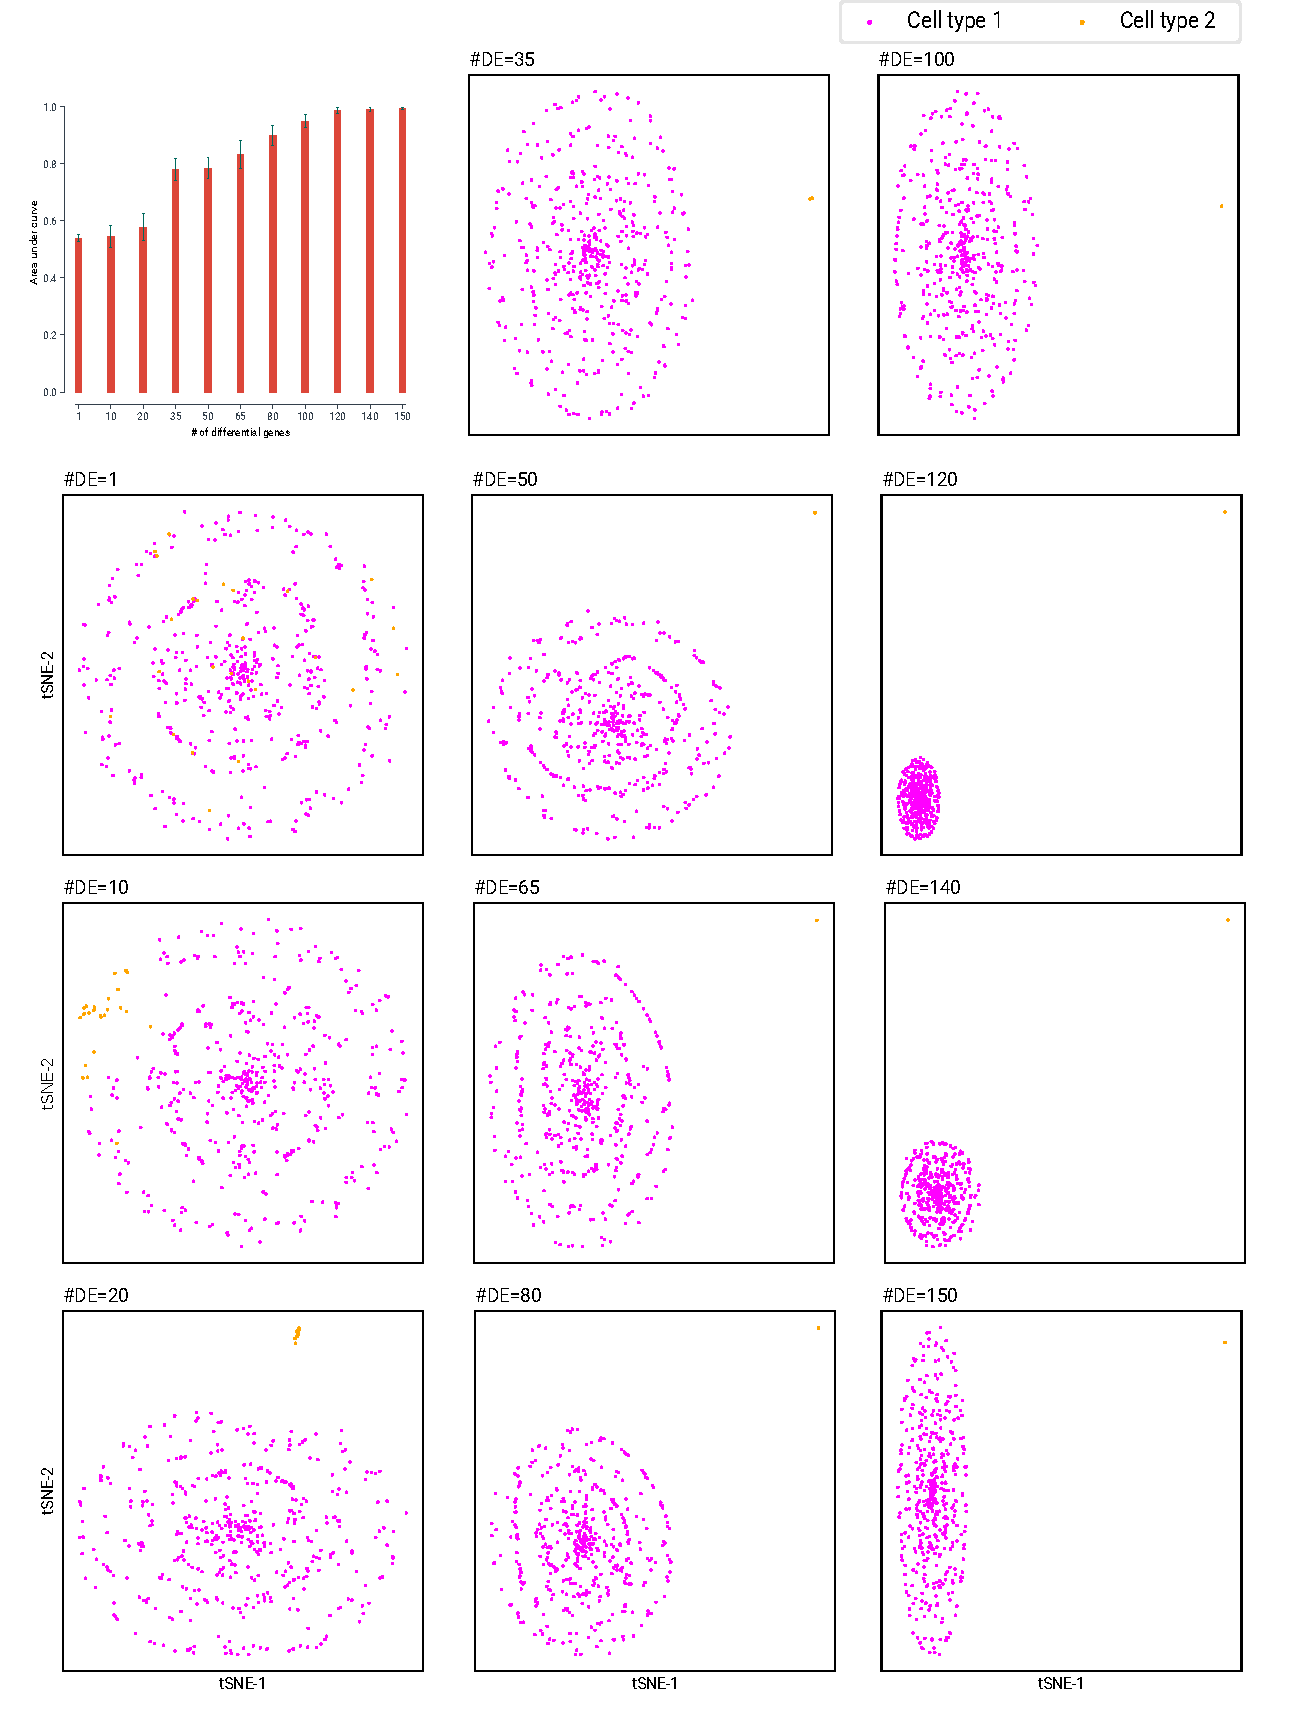
\includegraphics[width=0.9\textwidth]{simulate_panorama.pdf}
    \caption{
    % The sensitivity of DoRC to cell-type identities. 
    % On the scRNA-seq dataset \textit{Splatter\_500}, 
    % DoRC starts with recognizing the minor cell type correctly, 
    % as soon as the number of differentially expressed genes becomes adequate to give rise to a tiny cluster representing the minor cell
    % subpopulation. 
    % The top-left corner figure serves as a legend for the subsequent AUC plots. 
    % Each t-SNE and ROC plot pair serves as a representative of the 1000 repetitions of the experiment concerning a
    % specific number of differentially expressed genes. 
    % The AUC analysis is performed using cell-type annotations, 
    % and DoRC scores are assigned to individual cells.
    DoRC 对细胞类型特征敏感。
    % 在 scRNA-seq 数据集 \textit{Splatter\_500}上,
    % DoRC 从正确识别比例小的细胞类型开始,
    % 只要差异表达基因的数量变得足以产生一个代表小细胞亚群的微小簇。
    % 左上角图作为后续AUC图的图例。
    % 每个 t-SNE 和 ROC 图对对应为为 1000 次重复实验的一个代表结果,
    % 对应于一种特定数量的差异表达基因。
    % AUC 是使用各个细胞的类型标签和 DoRC 得分来计算到的。
    }
    \label{fig:simulate:roc}
\end{figure}

此外,由于 DoRC 和 FiRE 都可以给细胞做二元标注,
本文对其性能差异感到好奇。
在这个数据集中,我们考虑了 DoRC 和 FiRE 之间的 AUC、召回率、精度和 F1-score。
由于 F1-score 取决于召回率和精度,我们也包括这两个指标作为参考。
把细胞类型标注为真实标签, AUC 是用 DoRC 评分计算的。
而 F1-score是用 DoRC 评分产生的稀有度标注与 IQR 阈值标准获得的。
在两类实验中,直接构建一个混淆矩阵 (confusion matrix),其中的数值为真阳性 (TP)、假阳性 (FP)、真阴性 (TP)、假阴性 (FN)。
混淆矩阵上的精确率 Precision、召回率 Recall 计算如第 \ref{sec:locpcacmi} 章的公式 \ref{eq:precision}、\ref{eq:recall} 所示,
综合评价指标 F1-score 的计算如下面的公式 \ref{eq:f1score} 所示。
\begin{equation}
\label{eq:f1score}
\text{F1-score} = 2 \times \frac{\text{Precision} \times \text{Recall}}{ \text{Precision} + \text{Recall}}
\end{equation}

在总共 25 个稀有细胞中, DoRC 和 FiRE 都能正确检测出 23 个相同的稀有细胞。
DoRC 可以检测到其它 2 个稀有细胞和 1 个假阳性稀有细胞,
而 FiRE 未能识别出左边 2 个稀有细胞 (图 \ref{fig:simulate:venn_auc_f1} A)。
在这个数据集中, 阳性样品 (丰富细胞) 和阴性样品 (稀有细胞) 的数量是不平衡的。
这两种方法的 AUC 和精度基本没有变化,
但 DoRC 的召回率和 F1-score 均高于 FiRE (图 \ref{fig:simulate:venn_auc_f1} B)。
\begin{figure}[!htbp]
    \centering
    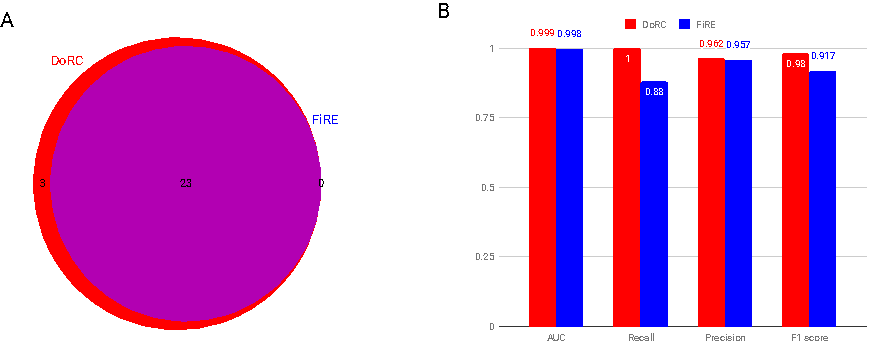
\includegraphics[width=0.9\textwidth]{plot_venn_dorcfire.pdf}
    \caption{
    % Comparison of DoRC and FiRE for rare cells detection in the dataset \textit{Splatter\_500}.
    % (A) Among all the 25 rare cells,  23 rare cells are all detected by DoRC and FiRE. 
    % DoRC could detect other 2 rare cells and 1 false positive rare cells, 
    % while FiRE failed to identify the left 2 rare cells.
    % (B) The AUC and precision of DoRC and FiRE are almost the same, while the Recall and  F1-score of DoRC is higher than FiRE.
    在 \textit{Splatter\_500}数据集上, DoRC 和 FiRE 对数据集中稀有细胞检测的比较。
    % (A) 在所有 25 个稀有细胞中, 23 个稀有细胞全部被 DoRC 和 FiRE 检测出来。
    % DoRC 可以检测到另外 2 个稀有细胞和 1 个假阳性稀有细胞,而 FiRE 则未能识别出剩下的 2 个稀有细胞。
    % (B) DoRC 和 FiRE 的 AUC 和精度几乎相同,而 DoRC 的 Recall 和 F1-score 高于 FiRE。
    }
    \label{fig:simulate:venn_auc_f1}
\end{figure}

DoRC 的核心算法孤立森林 (Isolation Forest) 的时间复杂度为 $O(ntlog\psi)$ \cite{liu2008isolation}。
其中 $n$、$t$ 和 $\psi$ 分别代表样本数、树的数目和每棵树的子样本数。
值得注意的是, DoRC 中的 Isolation Forest 在这种情况下没有训练的阶段。
该方法的参数我们使用默认值, t 设置为 100, $\psi$ 设置为 256。
因此, DoRC 的时间复杂度为 $O(n)$。
这个复杂度没有包括使用 RafClust 来确认稀有细胞的具体类型,
因为 FiRE 和 LOF 这两种方法也没有包含稀有细胞的类型细化这个步骤。

本文通过不断变化输入单细胞数据规模的大小,
分别统计出 DoRC、FiRE、GiniClust、LOF \cite{breunig2000lof} 和 RaceID 所消耗的时间,
如图 \ref{fig:timecomplexity} 所示。
测试机器为一台运行 GNU Linux/Ubuntu 16.04 操作系统 4.15.0-47-generic 内核的工作站上,
硬件配置如下: Intel(R) Xeon(R) Silver 4116 CPU @ 2.10GHz, 48 核, 64GB 内存。
DoRC 由 Python 实现,使用 scikit-learn包 (版本 0.20.2) \cite{pedregosa2011scikit}和 pyod包 (版本0.6.7)  \cite{zhao2019pyod}。
由于其它方法不能区分稀有细胞类型,在 DoRC 中我们也因此省略 RafClust 的稀有细胞类型细化的程序。
FiRE 从 \url{https://github.com/princethewinner/FiRE} 下载 (分支:master,最新提交的 abcba5b)。
因为 FiRE 的内核算法是用 C++ 编写的,我们在实验中使用的是其 Python 扩展分支。
GiniClust从 \url{https://github.com/lanjiangboston/GiniClust} 下载 (分支:master,最新提交 a442d45)。
我们在命令行界面直接使用 R 脚本,
额外的步骤包括 t-SNE 可视化和 DE 分析不计入时间对比评测中。
RaceID从 \url{https://github.com/dgrun/RaceID} 下载 (分支:master,最新提交 0a1e21c)。
LOF (local outlier factor) 是数据挖掘领域应用广泛的算法。
我们也直接使用 Pyod 包 (0.6.7版本) \cite{zhao2019pyod} 的 Python 实现 LOF。
值得注意的是, RaceID 和 GiniClust 仅输出了稀有细胞的二分标签预测,
而 DoRC、FiRE 和 LOF 则同时提供连续得分和二分标签预测。
\begin{figure}[!htbp]
    \centering
    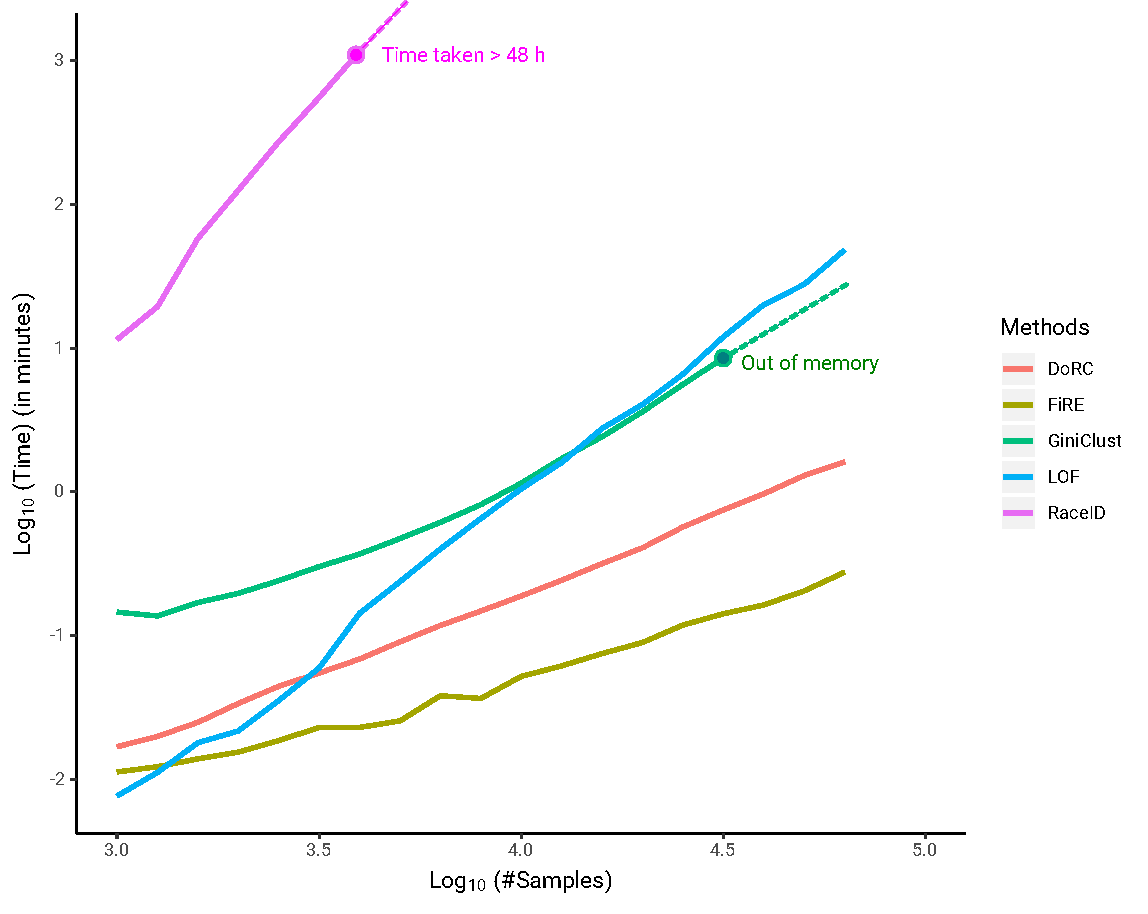
\includegraphics[width=0.9\textwidth]{Rplot_timecomplexity.pdf}
    \caption{
    % DoRC is fast. Execution time is recorded for DoRC, FiRE, GiniClust, LOF and RaceID, while varying the number of cells from 1k to ${\sim} 68$k
    DoRC的执行速度仅次于 FiRE。我们从 1k 到 ${\sim} 68$k 逐渐改变细胞的数目, 同时记录下 DoRC、FiRE、GiniClust、LOF 和 RaceID 的执行时间。    
    }
    \label{fig:timecomplexity}
\end{figure}
图 \ref{fig:timecomplexity} 展示了从 ${\sim}68$k scRNA-seq 数据中发现稀有细胞不同方法在不同细胞输入规模时所消耗的时间。 
GiniClust 和 RaceID 要么耗时,要么耗内存;
LOF 对输入数据规模非常敏感;
然而, DoRC 和 FiRE 都是非常快的,因为它们只需要不到 2 分钟就可以完成任务。
与 DoRC 相比, FiRE 的速度明显更快。
DoRC 的实现代码可在 GitHub 仓库 \url{https://github.com/chenxofhit/DoRC} 上获取,
本节相关的实验代码和相关数据集可以根据读者的要求提供。

\subsection{小结}

RafClust 是一种纯粹的无模型 (model free) 和数据驱动 (data driven) 的方法,
不需要其它的先验信息,如细胞或基因的群体结构、通路信息等。
本文使用多种相似性度量方法刻画细胞的特征,
使用随机森林回归模型来学习细胞与细胞之间的相似性矩阵,基于相似性矩阵后采用层次聚类来决定细胞的最终类别。
该方法既支持按照指定的细胞类别数聚类, 也可以让方法自主决定细胞的类别数,
还支持聚类结果的可视化和差异基因分析。
实验结果表明, 在十个单细胞数据集上, RafClust 在 ARI 上表现优于其它六种方法。

% 近来,单细胞转录组学大大改善了我们对细胞表型性质的理解,
% 并且,还加速了新细胞类型的发现。
% 这些新的细胞类型大多是罕见的,因为显然一种丰富的细胞类型如果在很长一段时间内不被我们观察到是很不可能的。
% 一个真正稀有的细胞类型只有通过分析成千上万的细胞才能被发现。
% 虽然过去几年的技术进步使我们能够进行超高通量的单细胞测序,
% 可扩展性的稀有细胞检测方法几乎不存在。
% DoRC 避免了使用聚类作为中间步骤,
% 因为聚类方法不仅耗时,但也不可能一次性完全绘制复杂组织中的细胞类型。

进一步地在 RafClust 方法的基础上, 本文提出了一种单细胞稀有细胞识别方法 DoRC。
该方法首先给每一个细胞表达图谱都单独给出了一个细胞稀有度分数。
然后通过 IQR 阈值, DoRC 也可以像 RaceID 和 GiniClust 一样提供二元标签预测。
DoRC 使用了 Isolation Forest 作为核心算法来实现这个功能。
Isolation Forest 是机器学习中被广泛研究、应用得很广的一种无监督的异常点 (离群值) 检测方法。
每个细胞的稀有度用其在相应的高维空间中的``异常点得分"来表示。
这种做法避免了直接使用聚类作为中间步骤,高效率地直接过滤出了稀有细胞。
DoRC 在 ${\sim}68$k 人血细胞单细胞表达谱上结合 RafClust 聚类方法,能准确识别出人血树突状细胞亚型。
此外,在其它两个模拟数据集上的实验表明, DoRC 可识别人工伪造的稀有细胞并且对细胞类型特征也很敏感。
实验还表明, DoRC 是可扩展的,而且速度很快。

单细胞测序从最初在转录组、基因组中的成功应用, 逐渐席卷到包括基因组、转录组、蛋白质组、表观组等各个组学。
单细胞 RNA-seq (scRNA-seq)、单细胞 ATAC-seq (scATAC-seq)、单细胞 Hi-C (scHi-c) 等已成为最重要的数据类型。
这些数据主要从 mRNA 表达量、染色质的三维结构、染色质可达性等不同方面反应了细胞的信息。
细胞异质性研究中可以结合这三种异构数据进行融合, RafClust 中构造细胞表达的特征矩阵是后续利用随机森林算法的基础,
这个步骤十分适合结合这三种异构数据直接构造细胞的特征矩阵。
后续,我们将关注融合单细胞多元组学的数据进行细胞的异质性研究, 以及在此基础上进一步发掘稀有细胞及其类型。

% 本章中,我们提出了一种高效准确的单细胞聚类方法 RafClust。
% 我们使用多种相似性度量方法刻画细胞的特征,
% 使用随机森林回归模型来学习细胞与细胞之间的相似性矩阵,基于相似性矩阵后采用层次聚类来决定细胞的最终类别。
% 实验结果表明, 在十个单细胞数据集上, RafClust 在 ARI 上表现优于其它六种方法。